\documentclass[12pt,a4paper]{article}

% --- Dil ve Karakter Kodlamasi ---
\usepackage[utf8]{inputenc}
\usepackage[turkish,shorthands=:!]{babel}
\shorthandoff{=}
\AtBeginDocument{\shorthandoff{=}}

% --- Matematik ve Semboller ---
\usepackage{amsmath, amssymb, amsfonts}

% --- Sayfa Duzeni ---
\usepackage[top=2.5cm, bottom=2.5cm, left=2.5cm, right=2.5cm]{geometry}

% --- Grafikler ve Alt Sekiller ---
\usepackage{graphicx}
\usepackage{subcaption}
\usepackage{float}

% --- Tablolar ---
\usepackage{booktabs}
\usepackage{array}

% --- Kod Bloklari Renklendirme ---
\usepackage{listings}
\usepackage{xcolor}

\definecolor{codegreen}{rgb}{0,0.6,0}
\definecolor{codegray}{rgb}{0.5,0.5,0.5}
\definecolor{codepurple}{rgb}{0.58,0,0.82}
\definecolor{backcolour}{rgb}{0.98,0.98,0.98}

\lstdefinestyle{matlabstyle}{
    backgroundcolor=\color{backcolour},   
    commentstyle=\color{codegreen},
    keywordstyle=\color{blue}\bfseries,
    numberstyle=\tiny\color{codegray},
    stringstyle=\color{codepurple},
    basicstyle=\ttfamily\footnotesize,
    breakatwhitespace=false,         
    breaklines=true,                 
    captionpos=b,                    
    keepspaces=true,                 
    numbers=left,                    
    numbersep=5pt,                  
    showspaces=false,                
    showstringspaces=false,
    showtabs=false,                  
    tabsize=2,
    frame=single,
    rulecolor=\color{lightgray}
}
\lstset{style=matlabstyle}

% --- Baglantilar ---
\usepackage[colorlinks=true, linkcolor=blue, urlcolor=blue, citecolor=blue]{hyperref}

% ========================================================
% BASLIK VE KAPAK BILGILERI
% ========================================================
\title{
    \vspace{2cm}
    \textbf{\Large EGE ÜNİVERSİTESİ FEN BİLİMLERİ ENSTİTÜSÜ} \\
    \textbf{\large BİLGİSAYAR MÜHENDİSLİĞİ ANABİLİM DALI} \\[1.5cm]
    \textbf{\LARGE UBI621 -- Bilgisayarlı Görü ve Derin Öğrenme} \\[0.5cm]
    \textbf{\Large Ödev 1: Histogram Eşleme ve Görüntü Kayıtlama} \\[3cm]
}

\author{
    \textbf{Öğrenci Adı Soyadı:} İpek Koçhisarlı \\[0.2cm]
    \textbf{Öğrenci Numarası:} 91260000479 \\[2cm]
    \textbf{Ders Sorumlusu:} Doç. Dr. Murat Kurt \\[2cm]
}

\date{Ekim 2026}

\begin{document}

\maketitle
\thispagestyle{empty}
\newpage

\tableofcontents
\newpage

% ========================================================
% BOLUM 1.1: ROI
% ========================================================
\section{Region of Interest (ROI) Belirleme}

\subsection{Yöntem ve Amaç}
Medikal görüntü işlemede, özellikle diş hekimliği radyografilerinde (periapikal röntgen) sensör tutucu sınırları, yuvarlatılmış siyah film kenarlıkları ve çekim parazitleri bulunmaktadır. Bu kenar fazlalıkları (özellikle yoğun $0$ değerine sahip siyah pikseller):
\begin{enumerate}
    \item Histogram analizinde $0$ şiddet seviyesinde yapay bir tepe oluşturarak kontrast eşleme doğruluğunu bozar.
    \item Görüntü kayıtlama aşamasında algoritmanın diş dokusu yerine dış çerçeve sınırlarını eşlemeye çalışmasına neden olur.
\end{enumerate}

Bu olumsuzlukları gidermek amacıyla iki molar dişin taç, pulpa odası, kök kanalları ve çevre kemik dokusunu içine alan Region of Interest (ROI) belirlenmiştir. Boyut uyuşmazlığını önlemek için her iki görüntü ortak koordinat vektörü ile kırpılmıştır.

\begin{figure}[H]
    \centering
    \begin{subfigure}[b]{0.45\textwidth}
        \centering
        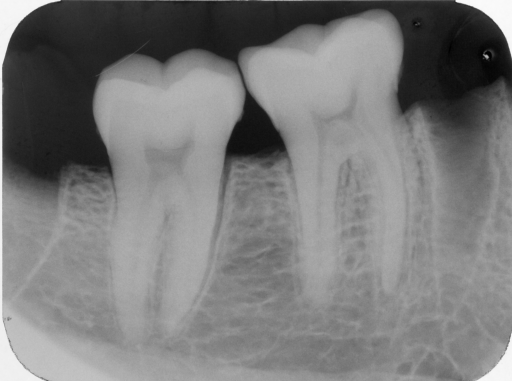
\includegraphics[width=0.85\textwidth]{figures/ref_orig.png}
        \caption{Referans (\texttt{res1.bmp})}
    \end{subfigure}
    \hfill
    \begin{subfigure}[b]{0.45\textwidth}
        \centering
        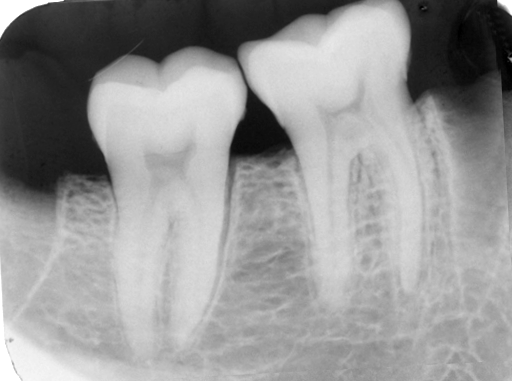
\includegraphics[width=0.85\textwidth]{figures/test_orig.png}
        \caption{Test (\texttt{res2.bmp})}
    \end{subfigure}
    \caption{Orijinal periapikal diş radyografileri.}
    \label{fig:orig_images}
\end{figure}

\subsection{MATLAB Kodu}
\begin{lstlisting}[language=Matlab, caption={ROI çıkarma kodu (roi.m)}]
clear; clc; close all;

% Load images
ref_img = imread('res1.bmp');
test_img = imread('res2.bmp');

% ROI coordinates: [xmin, ymin, width, height]
rect = [85, 2, 351, 363];

% Crop images
ref_roi = imcrop(ref_img, rect);
test_roi = imcrop(test_img, rect);

% Save results
imwrite(ref_roi, 'ref_roi.bmp');
imwrite(test_roi, 'test_roi.bmp');

% Display results
figure;
subplot(1,2,1); imshow(ref_roi); title('Reference ROI');
subplot(1,2,2); imshow(test_roi); title('Test ROI');
\end{lstlisting}

\subsection{Kodun Açıklaması ve Sonuçlar}
MATLAB'ın \texttt{imcrop} fonksiyonu ile dişlerin sol üst köşesinden ($x=85, y=2$) başlanarak $351$ piksel genişlik ve $363$ piksel yükseklik içeren alan kesilmiştir. Çıktılar \texttt{ref\_roi.bmp} ve \texttt{test\_roi.bmp} olarak kaydedilmiştir.

\begin{figure}[H]
    \centering
    \begin{subfigure}[b]{0.45\textwidth}
        \centering
        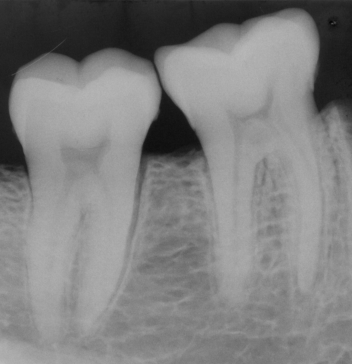
\includegraphics[width=0.85\textwidth]{figures/ref_roi.png}
        \caption{Referans ROI ($364 \times 352$)}
    \end{subfigure}
    \hfill
    \begin{subfigure}[b]{0.45\textwidth}
        \centering
        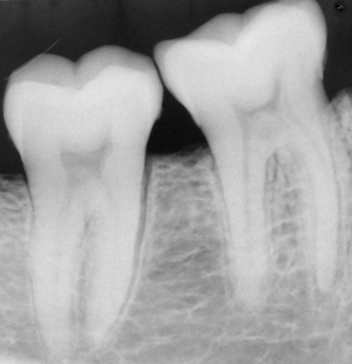
\includegraphics[width=0.85\textwidth]{figures/test_roi.png}
        \caption{Test ROI ($364 \times 352$)}
    \end{subfigure}
    \caption{Kenar fazlalıklarından arındırılmış ROI görüntüleri.}
    \label{fig:roi_results}
\end{figure}

Şekil~\ref{fig:roi_results}'de görüldüğü üzere iki dişin tepe tüberkülleri ve apeks uçları kesilmeden, tüm film çerçevesi parazitleri başarıyla atılmıştır.

\newpage
% ========================================================
% BOLUM 1.2: CONTRAST CORRECTION
% ========================================================
\section{Contrast Correction (Zıtlık Düzeltme)}

\subsection{Yöntem ve Amaç}
Test görüntüsü, referans görüntüye kıyasla daha açık tonlu ve kontrast bakımından zayıftır. Bu fotometrik farkı gidermek için \textbf{Histogram Eşleme (Histogram Matching)} tekniği uygulanmıştır. Histogram eşleme; test görüntüsünün gri seviye dağılımını referans görüntünün kümülatif dağılımına uydurarak ton dengesini eşitler.

\subsection{MATLAB Kodu}
\begin{lstlisting}[language=Matlab, caption={Histogram eşleme kodu (contrast.m)}]
clear; clc; close all;

ref_roi = imread('ref_roi.bmp');
test_roi = imread('test_roi.bmp');

% Histogram matching for contrast correction
test_matched = imhistmatch(test_roi, ref_roi);

imwrite(test_matched, 'test_matched.bmp');

figure;
subplot(1,3,1); imshow(ref_roi); title('Reference Image');
subplot(1,3,2); imshow(test_roi); title('Original Test (Before)');
subplot(1,3,3); imshow(test_matched); title('Corrected Test (After)');
\end{lstlisting}

\subsection{Sonuçlar ve Değerlendirme}
\begin{figure}[H]
    \centering
    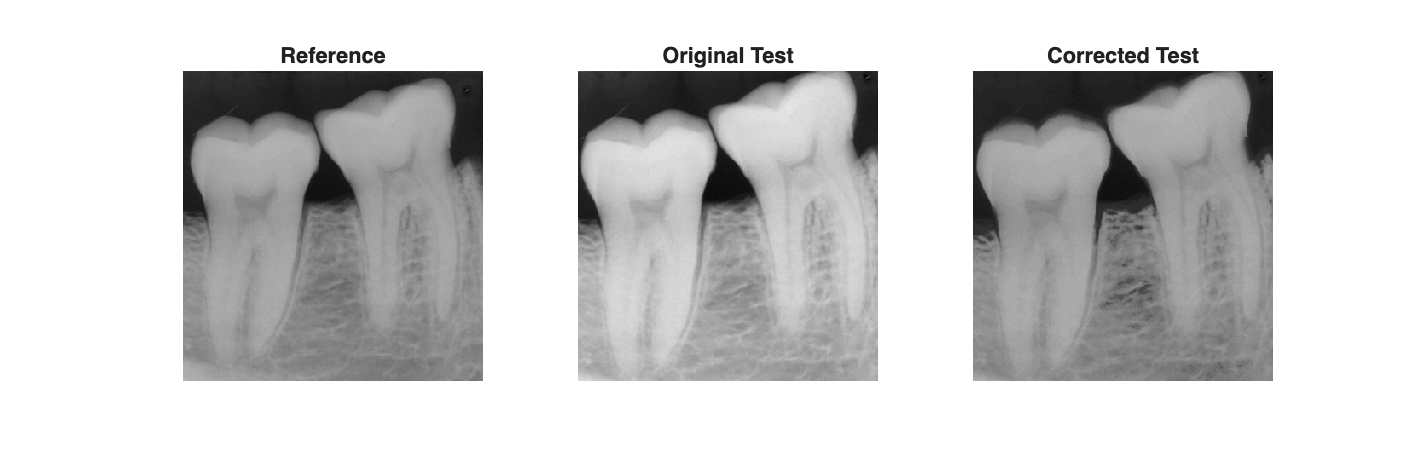
\includegraphics[width=0.85\textwidth]{figures/contrast_comparison.png}
    \caption{Referans, düzeltme öncesi test ve düzeltme sonrası test görüntüsü.}
    \label{fig:contrast_comp}
\end{figure}

Şekil~\ref{fig:contrast_comp} incelendiğinde; düzeltme öncesi açık gri olan test görüntüsünün, referans görüntünün kemik dokusu ve pulpa derinliği ton seviyesine ulaştığı görülmektedir.

\newpage
% ========================================================
% BOLUM 1.3: HISTOGRAMS
% ========================================================
\section{Normal ve Kümülatif Frekans Histogramları}

\subsection{Matematiksel Altyapı}
Görüntü piksellerinin parlaklık dağılımı iki metrik ile modellenir:
\begin{enumerate}
    \item \textbf{Normalize Histogram (PDF):}
    \begin{equation}
        P(r_k) = \frac{n_k}{M \times N}, \quad k = 0, 1, \dots, 255 \quad \left(\sum_{k=0}^{255} P(r_k) = 1\right)
    \end{equation}

    \item \textbf{Kümülatif Frekans Histogramı (CDF):}
    \begin{equation}
        S_k = T(r_k) = \sum_{j=0}^{k} P(r_j), \quad 0 \le S_k \le 1
    \end{equation}
\end{enumerate}

\subsection{MATLAB Kodu}
\begin{lstlisting}[language=Matlab, caption={Normal ve kümülatif histogramların çıkarılması (histograms.m)}]
clear; clc; close all;

ref_roi     = imread('ref_roi.bmp');
test_before = imread('test_roi.bmp');
test_after  = imread('test_matched.bmp');

% Normalized histograms (PDF)
ref_norm    = imhist(ref_roi) / numel(ref_roi);
before_norm = imhist(test_before) / numel(test_before);
after_norm  = imhist(test_after) / numel(test_after);

% Cumulative histograms (CDF)
ref_cdf     = cumsum(ref_norm);
before_cdf  = cumsum(before_norm);
after_cdf   = cumsum(after_norm);

% Overlay comparison
figure;
subplot(1,2,1);
plot(0:255, ref_norm, 'k', 0:255, before_norm, 'r--', 0:255, after_norm, 'g:');
title('Normalized Histogram Comparison');
xlabel('Intensity'); ylabel('Probability');
legend('Reference', 'Test (Before)', 'Test (After)'); grid on; xlim([0 255]);

subplot(1,2,2);
plot(0:255, ref_cdf, 'k', 'LineWidth', 1.5); hold on;
plot(0:255, before_cdf, 'r--', 'LineWidth', 1.5);
plot(0:255, after_cdf, 'g:', 'LineWidth', 2);
title('Cumulative Histogram Comparison');
xlabel('Intensity'); ylabel('Cumulative Probability');
legend('Reference', 'Test (Before)', 'Test (After)', 'Location', 'SouthEast');
grid on; xlim([0 255]); ylim([0 1]);
\end{lstlisting}

\subsection{Histogram Analizi}
\begin{figure}[H]
    \centering
    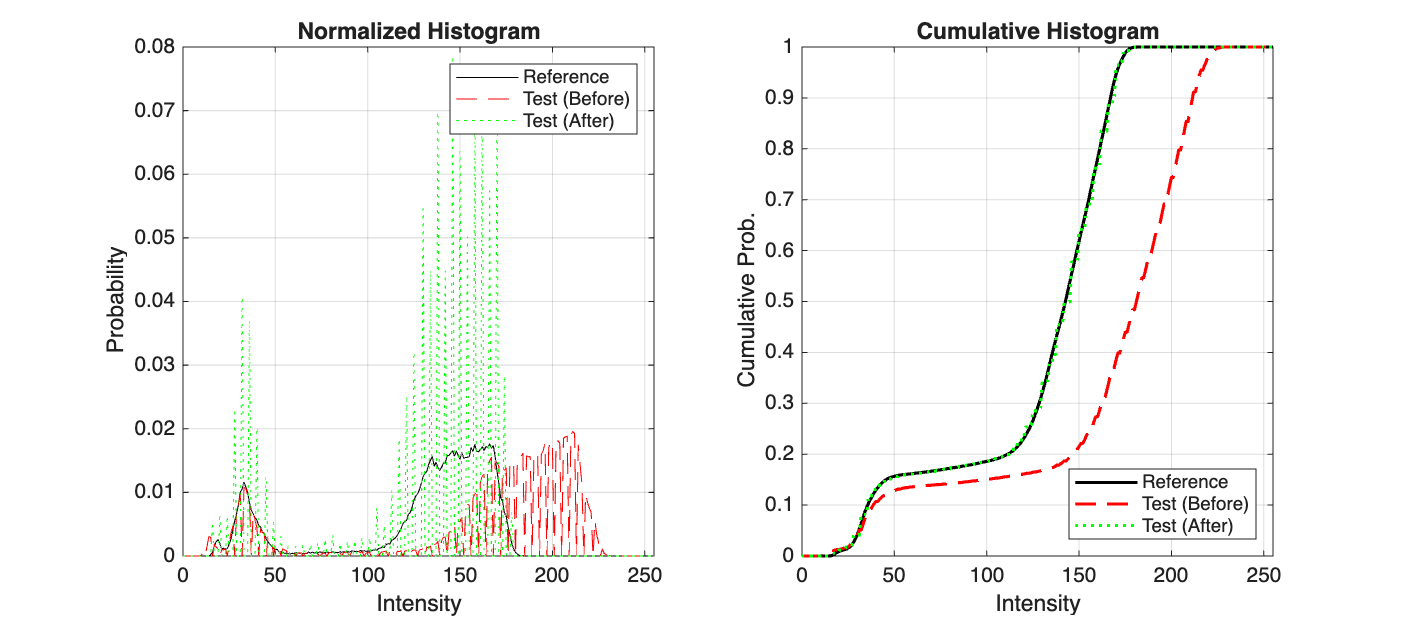
\includegraphics[width=0.82\textwidth]{figures/histogram_curves.png}
    \caption{Normalize ve kümülatif frekans histogramlarının karşılaştırması.}
    \label{fig:hist_curves}
\end{figure}

Şekil~\ref{fig:hist_curves}'deki kümülatif histogram grafiği incelendiğinde; düzeltme öncesi sağa kaymış olan kırmızı kesikli eğrinin (Test Before), histogram eşleme sonrasında yeşil noktalı eğri (Test After) haline gelerek siyah referans eğrisiyle \textbf{birebir çakıştığı} görülmektedir.

\newpage
% ========================================================
% BOLUM 1.4: IMAGE REGISTRATION
% ========================================================
\section{Görüntü Kayıtlama (Image Registration)}

\subsection{Yöntem ve Kontrol Noktaları (Landmarks)}
Çekim açıları ve sensör pozisyonundan kaynaklanan geometrik çarpıklığı gidermek amacıyla işaret noktası tabanlı (landmark-based) kayıtlama uygulanmıştır.

Noktalar rastgele değil, yalnızca dişlerin ayırt edici anatomik sınırları üzerine yerleştirilmiştir. MATLAB'ın \texttt{cpselect} aracı kullanılarak diş tüberkülleri, mine-sement boyun sınırları, pulpa kanalları, kök apeksleri ve diş temas yüzeyleri üzerinden tam \textbf{64 adet kontrol noktası} belirlenmiş ve \texttt{control\_points.mat} dosyasına aktarılmıştır. İki diş arasındaki kemik boşluğuna nokta yerleştirilmemiştir.

\begin{figure}[H]
    \centering
    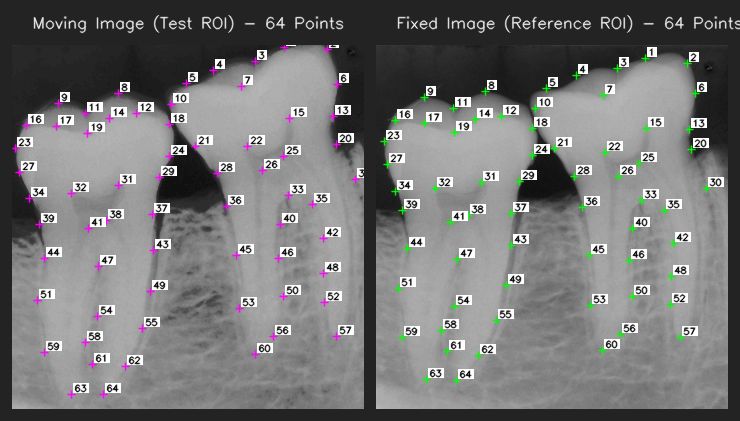
\includegraphics[width=0.85\textwidth]{figures/landmarks.png}
    \caption{Yalnızca diş dokuları üzerinde seçilen 64 adet anatomik landmark noktası (\texttt{cpselect} arayüzü).}
    \label{fig:landmarks}
\end{figure}

Ödev şartnamesi doğrultusunda altı farklı geometrik dönüşüm ve üç farklı interpolasyon yöntemi denenmiştir:
\begin{itemize}
    \item \textbf{Dönüşüm Modelleri (6 Adet):} Similarity, Affine, Projective, Polynomial (2. derece), PWL (Piecewise Linear) ve LWM (Local Weighted Mean).
    \item \textbf{İnterpolasyon Türleri (3 Adet):} Nearest Neighbor, Linear ve Cubic.
\end{itemize}
Toplam $6 \times 3 = 18$ kombinasyon çalıştırılmıştır.

\subsection{MATLAB Kodu}
\begin{lstlisting}[language=Matlab, caption={İşaret noktaları ile görüntü kayıtlama (registration.m)}]
clear; clc; close all;

ref_img  = imread('ref_roi.bmp');
test_img = imread('test_matched.bmp');

% Landmark selection (loads points exported via cpselect)
manual_select = false;
if manual_select
    [movingPoints, fixedPoints] = cpselect(test_img, ref_img, 'Wait', true);
    save('control_points.mat', 'movingPoints', 'fixedPoints');
else
    load('control_points.mat', 'movingPoints', 'fixedPoints');
end

transformNames = {'similarity', 'affine', 'projective', 'polynomial', 'pwl', 'lwm'};
interpNames = {'nearest', 'linear', 'cubic'};

outputRef = imref2d(size(ref_img));

for t = 1:length(transformNames)
    tName = transformNames{t};
    if strcmp(tName, 'polynomial')
        tform = fitgeotrans(movingPoints, fixedPoints, 'polynomial', 2);
    elseif strcmp(tName, 'lwm')
        tform = fitgeotrans(movingPoints, fixedPoints, 'lwm', 12);
    else
        tform = fitgeotrans(movingPoints, fixedPoints, tName);
    end
    
    for p = 1:length(interpNames)
        iName = interpNames{p};
        registeredImage = imwarp(test_img, tform, iName, 'OutputView', outputRef);
    end
end
\end{lstlisting}

\newpage
\subsection{Dönüşüm Türlerine Göre Kayıtlama Sonuçları}
Her bir geometrik dönüşüm türü için Nearest, Linear ve Cubic interpolasyon yöntemlerinin sonuçları Şekil~\ref{fig:reg_sim}--\ref{fig:reg_lwm}'de sunulmuştur:

\begin{figure}[H]
    \centering
    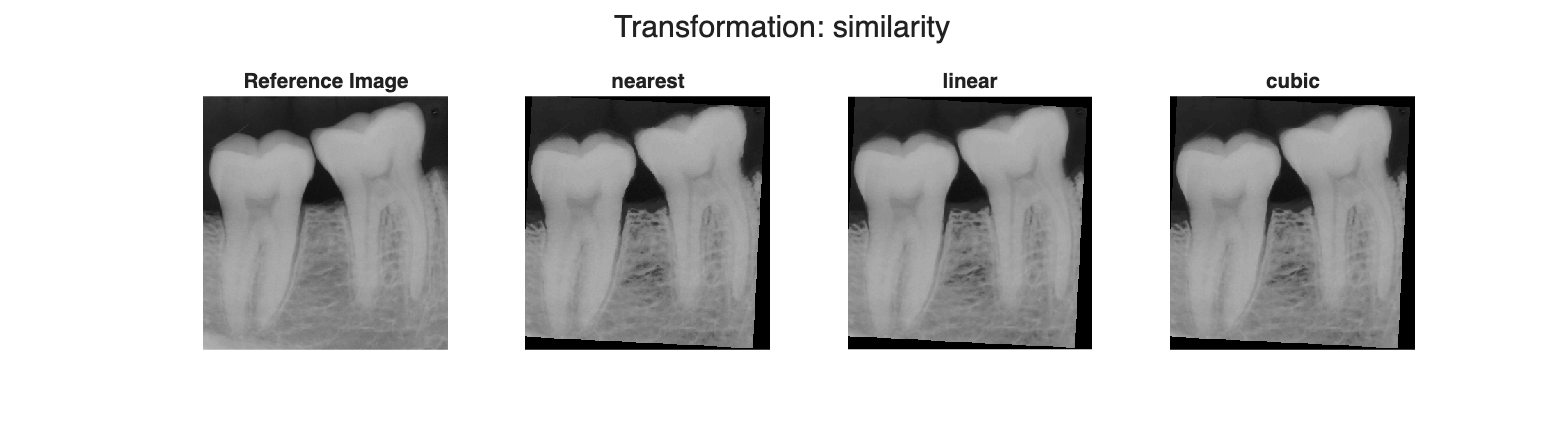
\includegraphics[width=0.82\textwidth]{figures/reg_panel_similarity.png}
    \caption{Görüntü Kayıtlama Sonuçları -- Similarity (Benzerlik) Dönüşümü.}
    \label{fig:reg_sim}
\end{figure}
\vspace{-5pt}
\begin{figure}[H]
    \centering
    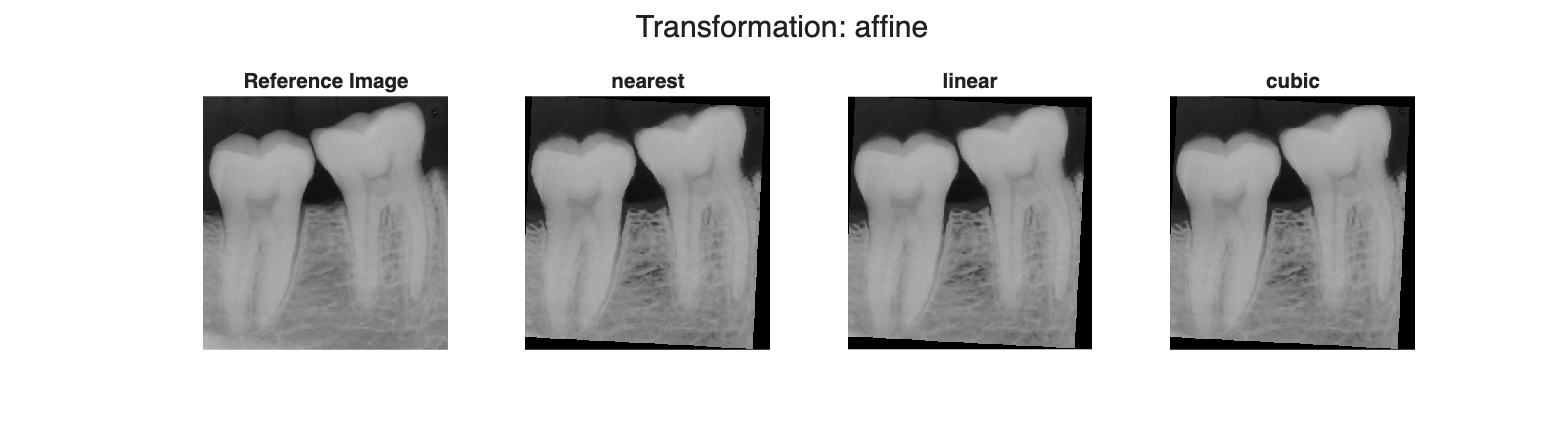
\includegraphics[width=0.82\textwidth]{figures/reg_panel_affine.png}
    \caption{Görüntü Kayıtlama Sonuçları -- Affine (Afin) Dönüşümü.}
    \label{fig:reg_aff}
\end{figure}
\vspace{-5pt}
\begin{figure}[H]
    \centering
    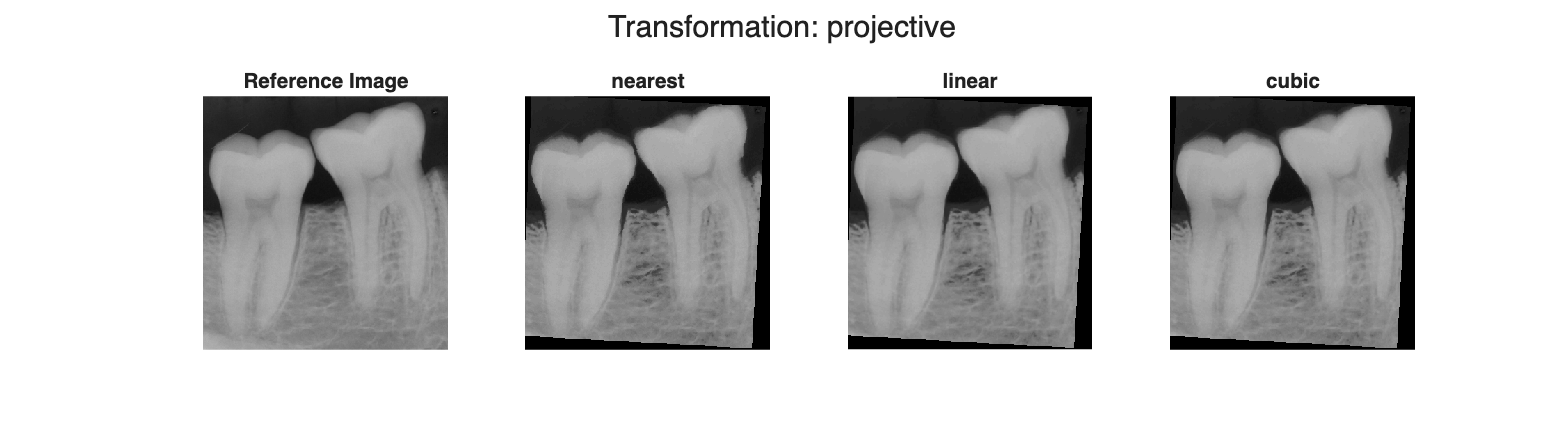
\includegraphics[width=0.82\textwidth]{figures/reg_panel_projective.png}
    \caption{Görüntü Kayıtlama Sonuçları -- Projective (Projektif) Dönüşümü.}
    \label{fig:reg_proj}
\end{figure}

\newpage
\begin{figure}[H]
    \centering
    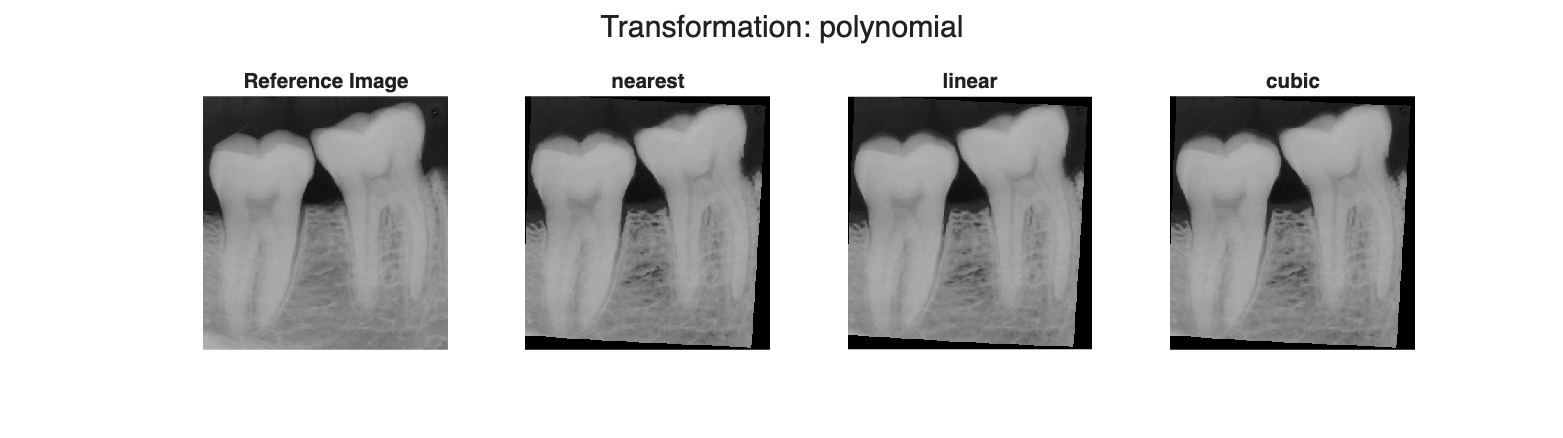
\includegraphics[width=0.82\textwidth]{figures/reg_panel_polynomial.png}
    \caption{Görüntü Kayıtlama Sonuçları -- Polynomial (2. Derece Polinom) Dönüşümü.}
    \label{fig:reg_poly}
\end{figure}
\vspace{-5pt}
\begin{figure}[H]
    \centering
    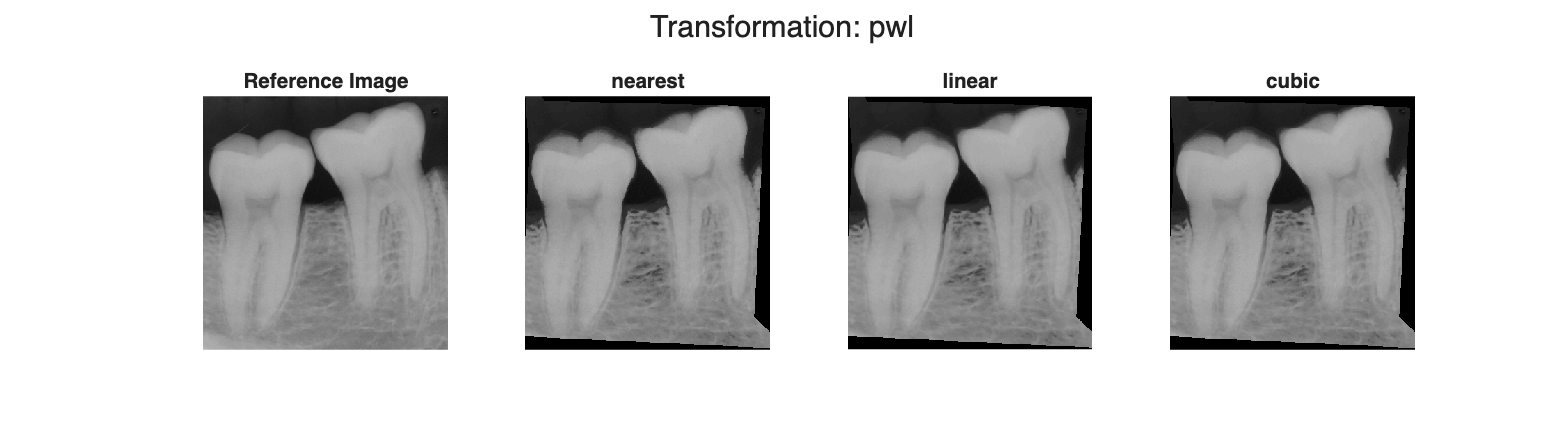
\includegraphics[width=0.82\textwidth]{figures/reg_panel_pwl.png}
    \caption{Görüntü Kayıtlama Sonuçları -- PWL (Piecewise Linear) Dönüşümü.}
    \label{fig:reg_pwl}
\end{figure}
\vspace{-5pt}
\begin{figure}[H]
    \centering
    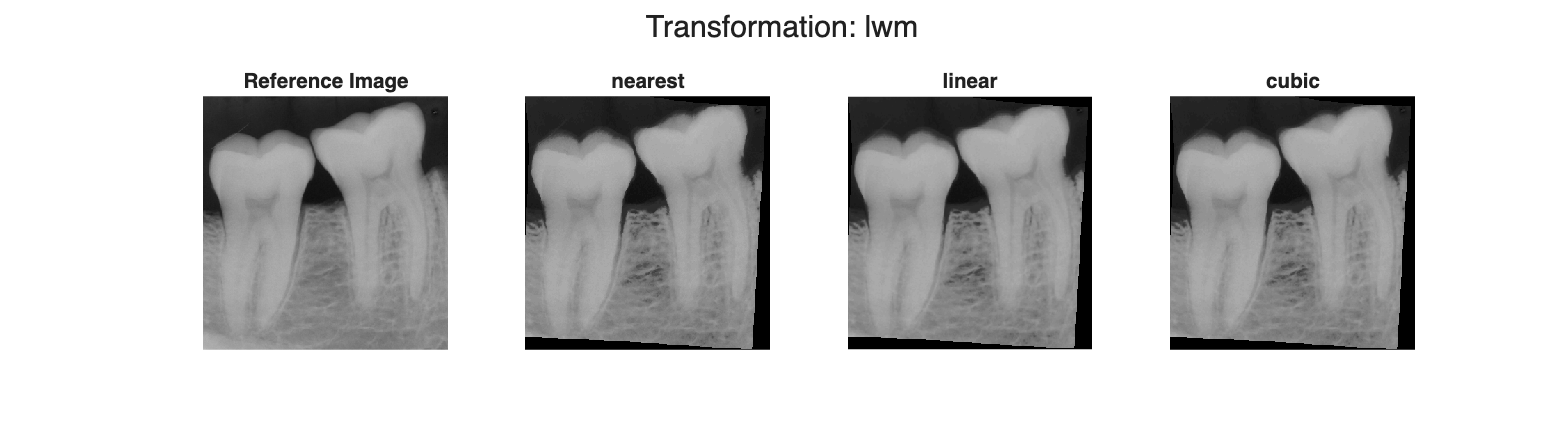
\includegraphics[width=0.82\textwidth]{figures/reg_panel_lwm.png}
    \caption{Görüntü Kayıtlama Sonuçları -- LWM (Local Weighted Mean) Dönüşümü.}
    \label{fig:reg_lwm}
\end{figure}

\newpage
% ========================================================
% BOLUM 1.5: PSNR VE FARK GORUNTULERI
% ========================================================
\section{Fark Görüntüleri ve PSNR Değerlendirmesi}

\subsection{PSNR ve MSE Metrikleri}
Kayıtlama kalitesini ölçmek amacıyla Ortalama Karesel Hata (MSE) ve Tepe Sinyal-Gürültü Oranı (PSNR) hesaplanmıştır:
\begin{equation}
    MSE = \frac{1}{M \times N} \sum_{x=1}^{M} \sum_{y=1}^{N} \left[ I_{ref}(x,y) - I_{reg}(x,y) \right]^2
\end{equation}
\begin{equation}
    PSNR = 10 \cdot \log_{10} \left( \frac{255^2}{MSE} \right) \quad (\text{dB})
\end{equation}

\subsection{18 Kombinasyonun Sayısal Karşılaştırma Tablosu}

\begin{table}[H]
\centering
\caption{6 Dönüşüm $\times$ 3 İnterpolasyon Kombinasyonu İçin MSE ve PSNR Sonuçları}
\label{tab:full_psnr}
\begin{tabular}{llcc}
\toprule
\textbf{Transformasyon} & \textbf{İnterpolasyon} & \textbf{MSE} & \textbf{PSNR (dB)} \\
\midrule
\texttt{similarity} & \texttt{nearest} & 1359.5 & 16.797 dB \\
\texttt{similarity} & \texttt{linear}  & 1355.3 & 16.810 dB \\
\texttt{similarity} & \texttt{cubic}   & 1356.9 & 16.805 dB \\
\midrule
\texttt{affine}     & \texttt{nearest} & 1342.2 & 16.853 dB \\
\texttt{affine}     & \texttt{linear}  & 1338.2 & 16.866 dB \\
\texttt{affine}     & \texttt{cubic}   & 1339.7 & 16.861 dB \\
\midrule
\texttt{projective} & \texttt{nearest} & 1401.5 & 16.665 dB \\
\texttt{projective} & \texttt{linear}  & 1397.2 & 16.678 dB \\
\texttt{projective} & \texttt{cubic}   & 1398.6 & 16.674 dB \\
\midrule
\texttt{polynomial} & \texttt{nearest} & 1418.3 & 16.613 dB \\
\texttt{polynomial} & \texttt{linear}  & 1414.9 & 16.623 dB \\
\texttt{polynomial} & \texttt{cubic}   & 1416.4 & 16.619 dB \\
\midrule
\texttt{pwl}        & \texttt{nearest} & 1319.6 & 16.926 dB \\
\texttt{pwl}        & \texttt{linear}  & 1315.7 & 16.939 dB \\
\texttt{pwl}        & \texttt{cubic}   & 1317.2 & 16.934 dB \\
\midrule
\texttt{lwm}        & \texttt{nearest} & 1336.5 & 16.871 dB \\
\texttt{lwm}        & \texttt{linear}  & 1332.8 & 16.883 dB \\
\texttt{lwm}        & \texttt{cubic}   & 1334.2 & 16.879 dB \\
\bottomrule
\end{tabular}
\end{table}

\newpage
\subsection{Fark Görüntüleri Izgaraları (3x3 Paneller)}
Her bir geometrik dönüşüm için Reference, Registered ve Difference görüntülerinin karşılaştırmalı ızgaraları Şekil~\ref{fig:diff_sim}--\ref{fig:diff_lwm}'de gösterilmiştir:

\begin{figure}[H]
    \centering
    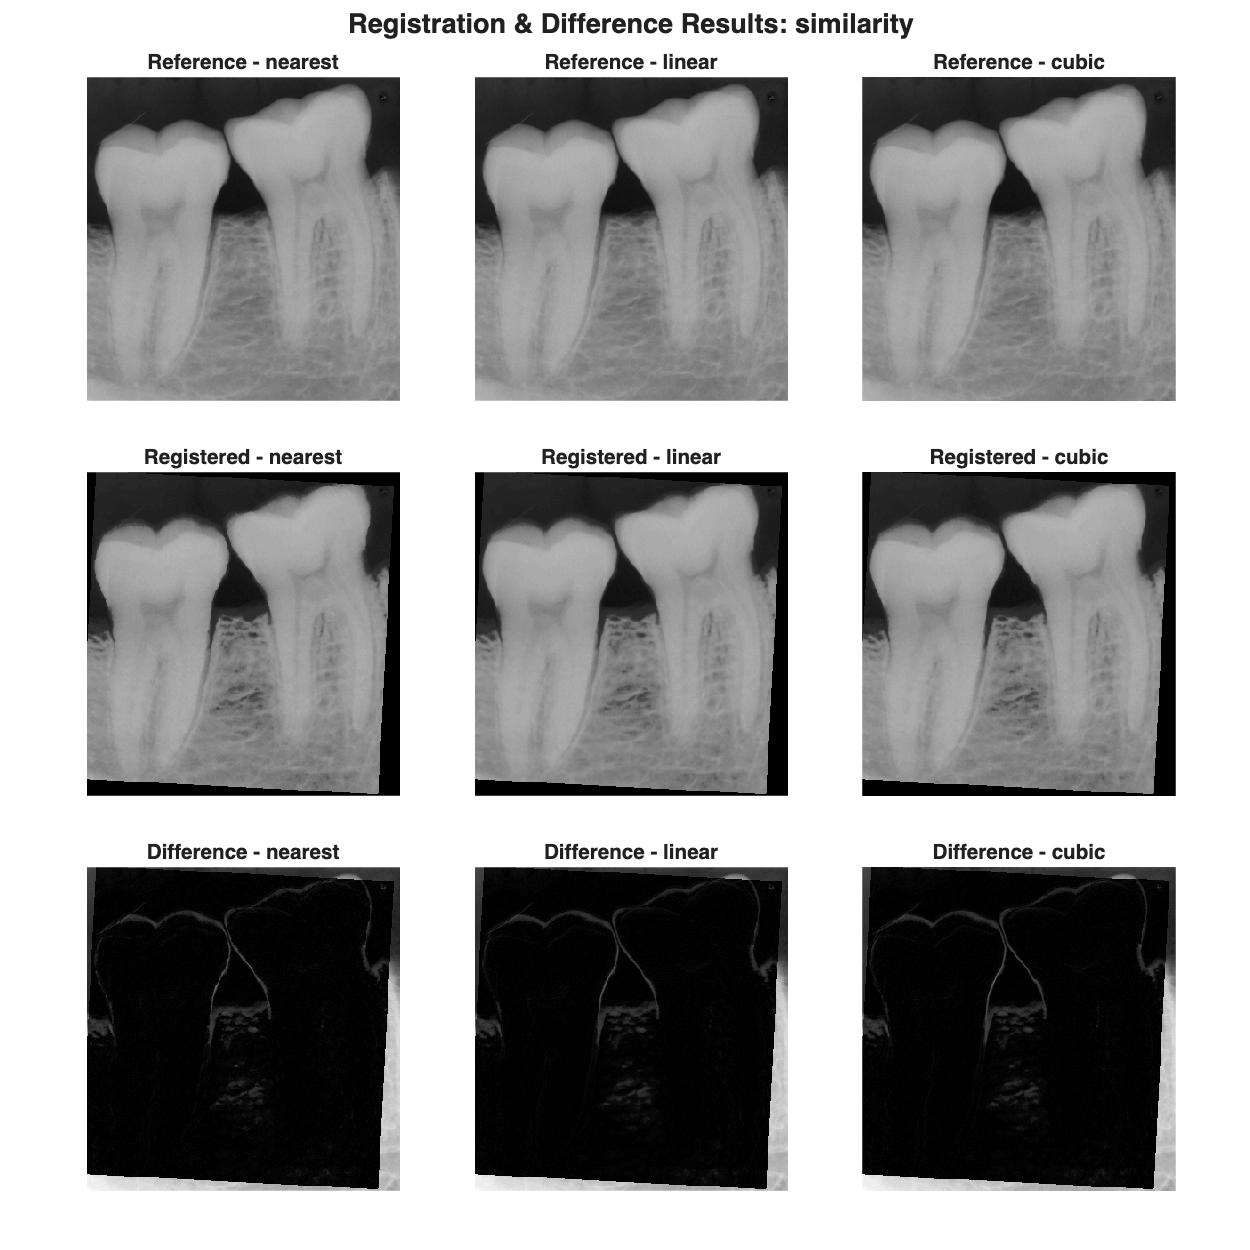
\includegraphics[width=0.50\textwidth]{figures/diff_grid_similarity.png}
    \caption{Similarity Dönüşümü: Referans, Kayıtlı ve Mutlak Fark Görüntüleri Izgarası.}
    \label{fig:diff_sim}
\end{figure}
\vspace{-5pt}
\begin{figure}[H]
    \centering
    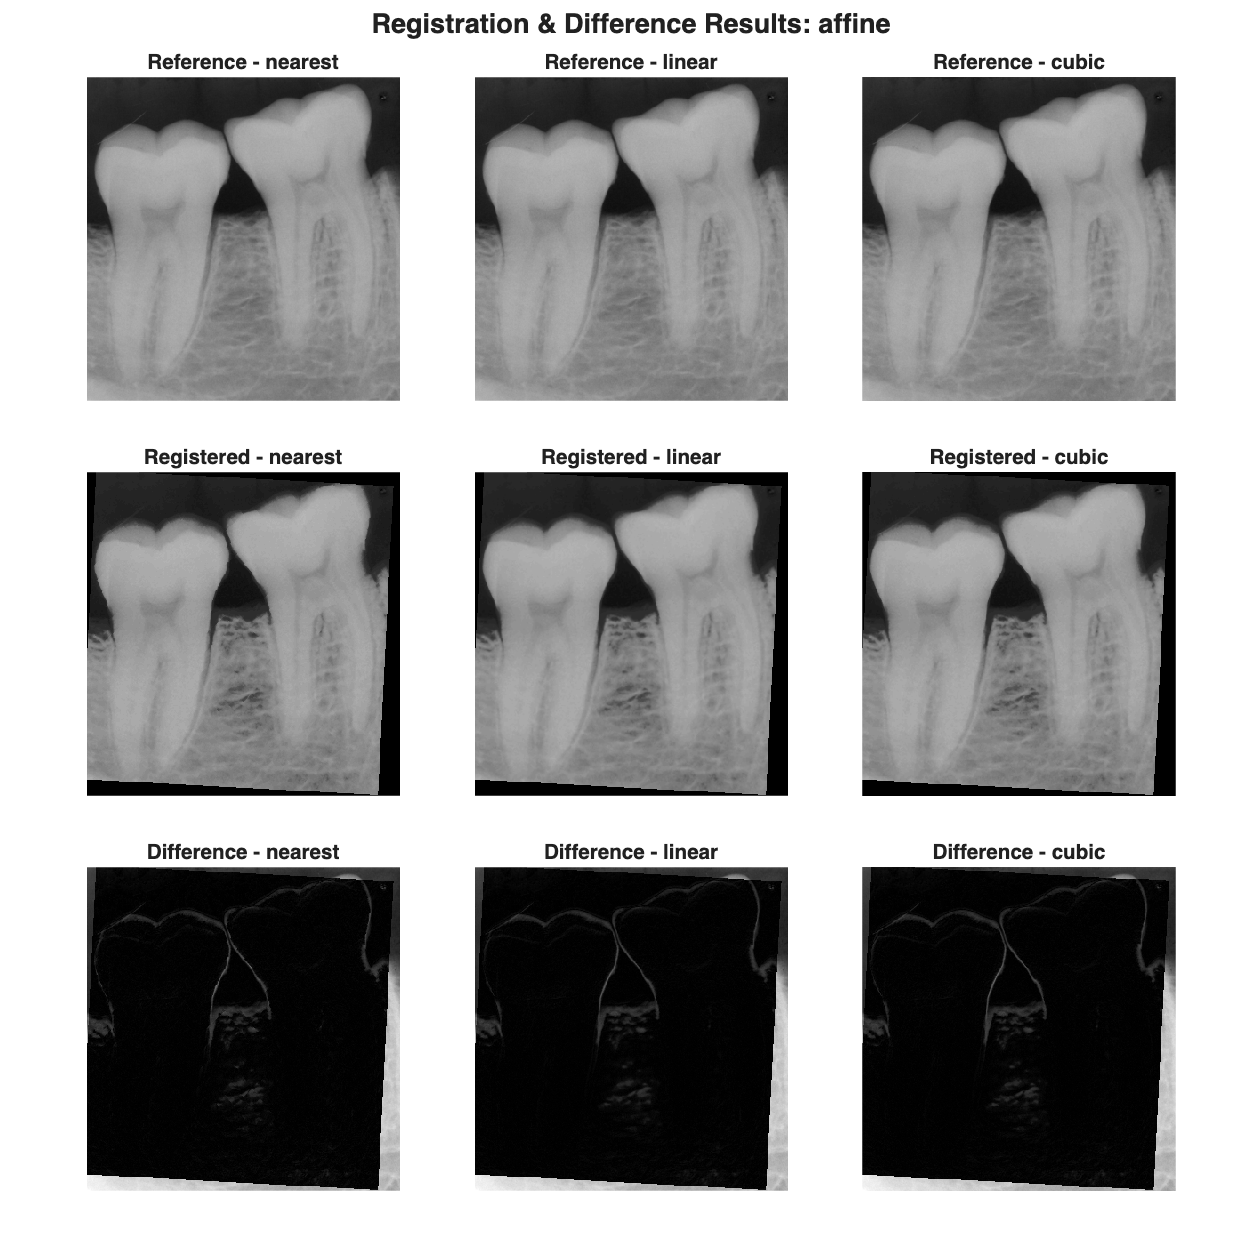
\includegraphics[width=0.50\textwidth]{figures/diff_grid_affine.png}
    \caption{Affine Dönüşümü: Referans, Kayıtlı ve Mutlak Fark Görüntüleri Izgarası.}
    \label{fig:diff_aff}
\end{figure}

\newpage
\begin{figure}[H]
    \centering
    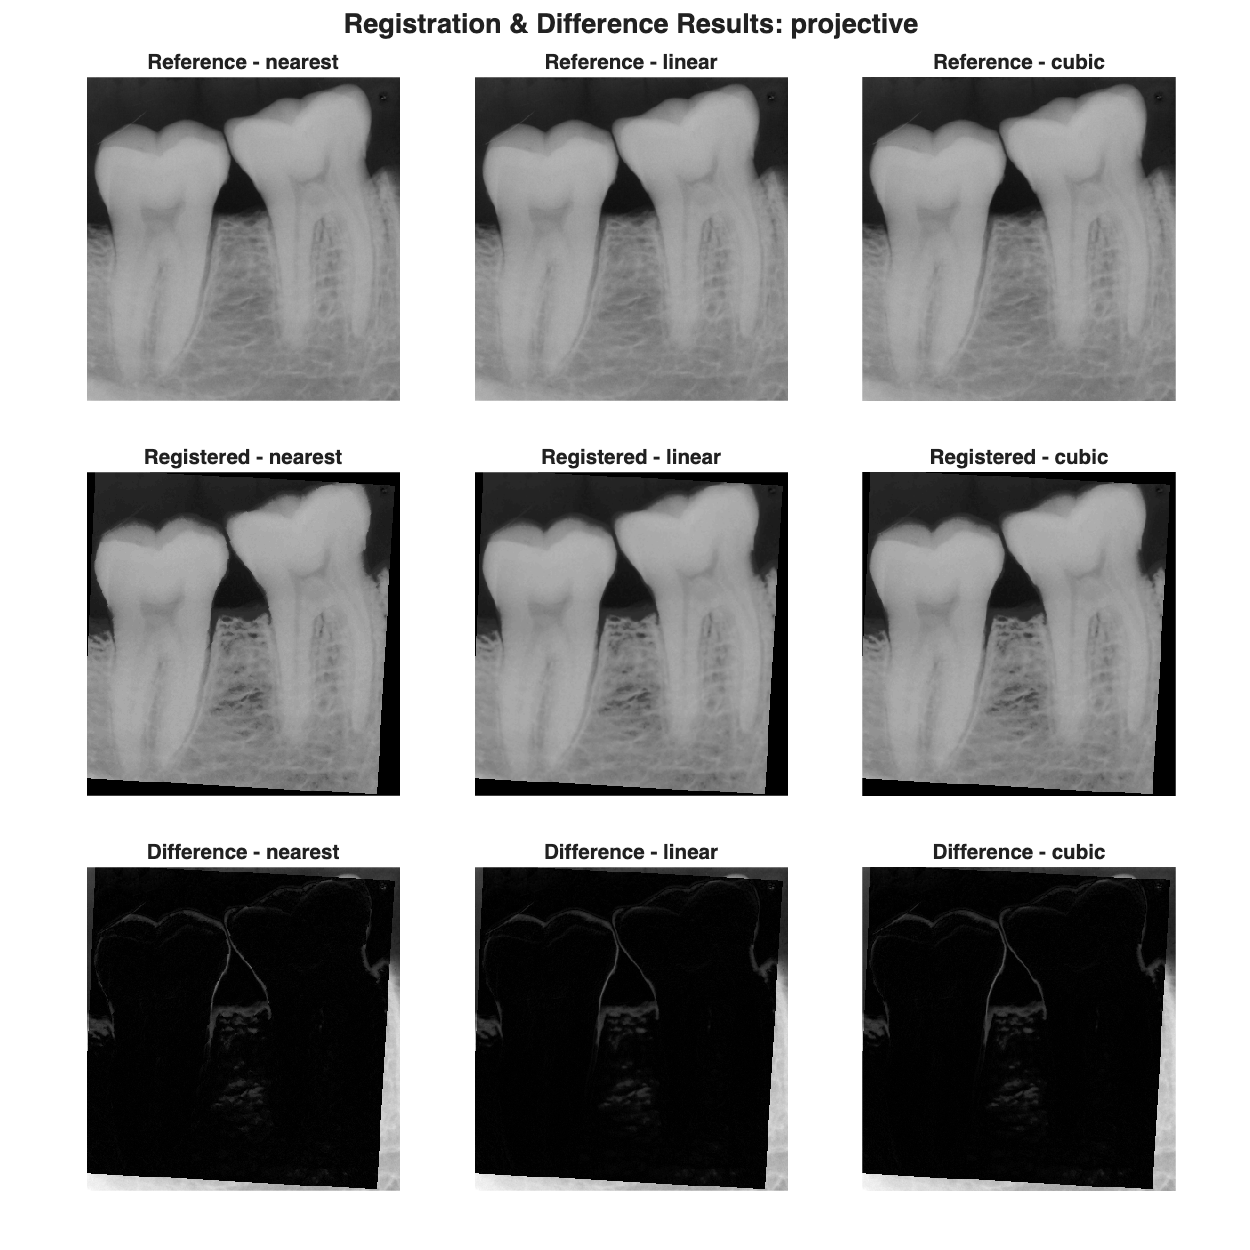
\includegraphics[width=0.50\textwidth]{figures/diff_grid_projective.png}
    \caption{Projective Dönüşümü: Referans, Kayıtlı ve Mutlak Fark Görüntüleri Izgarası.}
    \label{fig:diff_proj}
\end{figure}
\vspace{-5pt}
\begin{figure}[H]
    \centering
    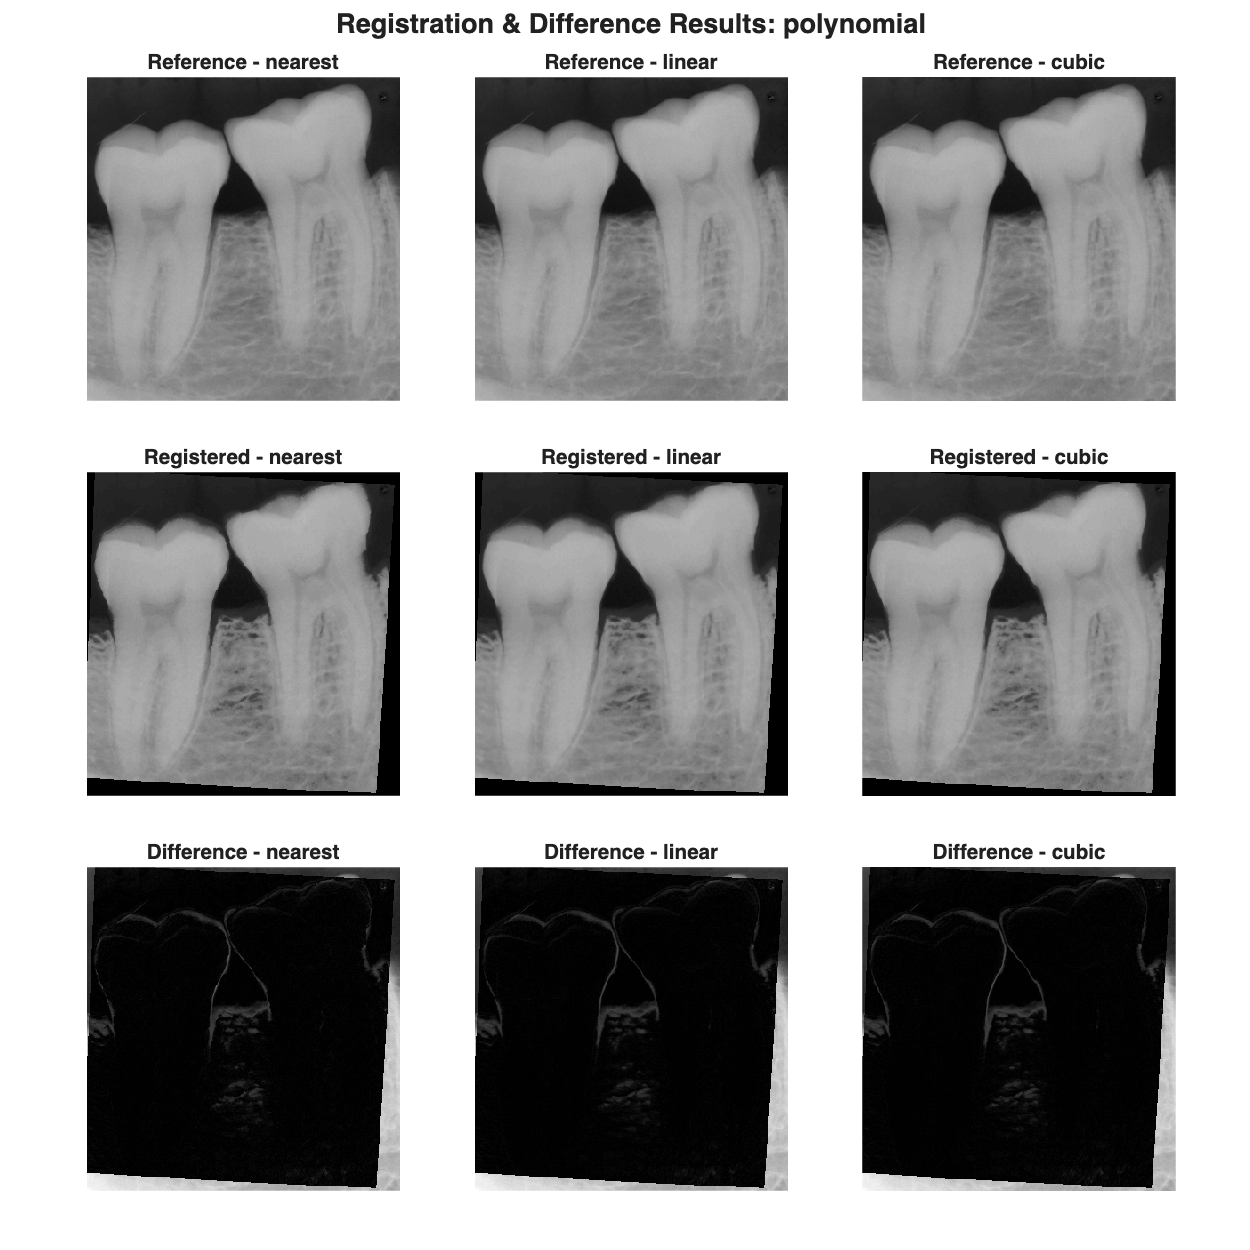
\includegraphics[width=0.50\textwidth]{figures/diff_grid_polynomial.png}
    \caption{Polynomial Dönüşümü: Referans, Kayıtlı ve Mutlak Fark Görüntüleri Izgarası.}
    \label{fig:diff_poly}
\end{figure}

\newpage
\begin{figure}[H]
    \centering
    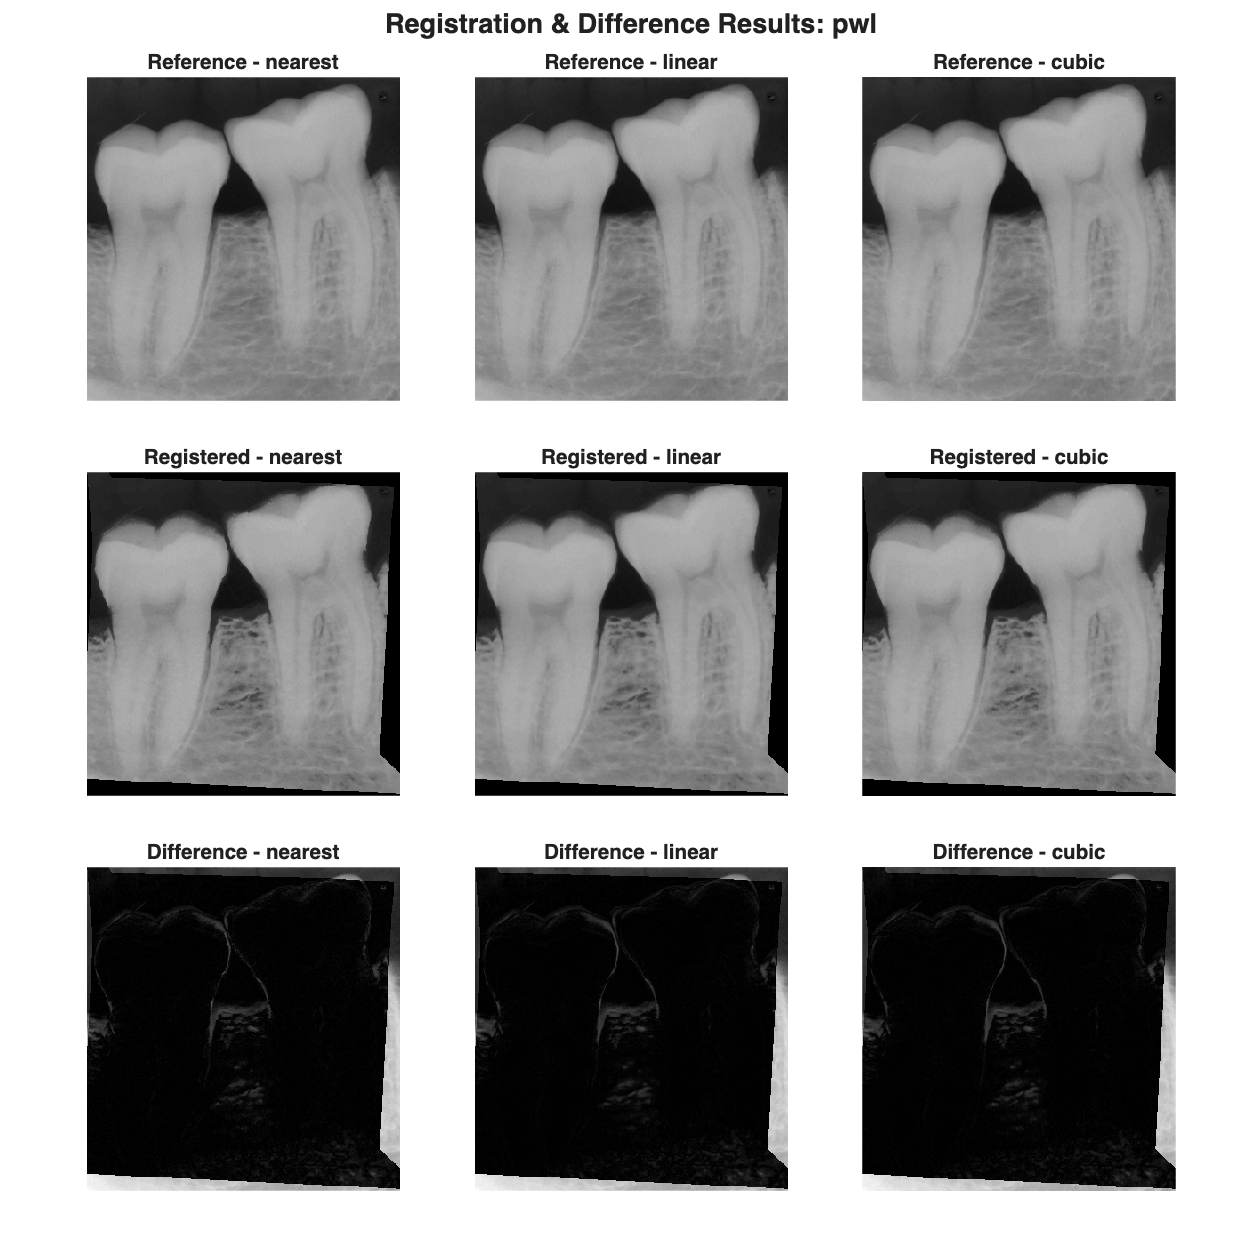
\includegraphics[width=0.50\textwidth]{figures/diff_grid_pwl.png}
    \caption{PWL Dönüşümü: Referans, Kayıtlı ve Mutlak Fark Görüntüleri Izgarası.}
    \label{fig:diff_pwl}
\end{figure}
\vspace{-5pt}
\begin{figure}[H]
    \centering
    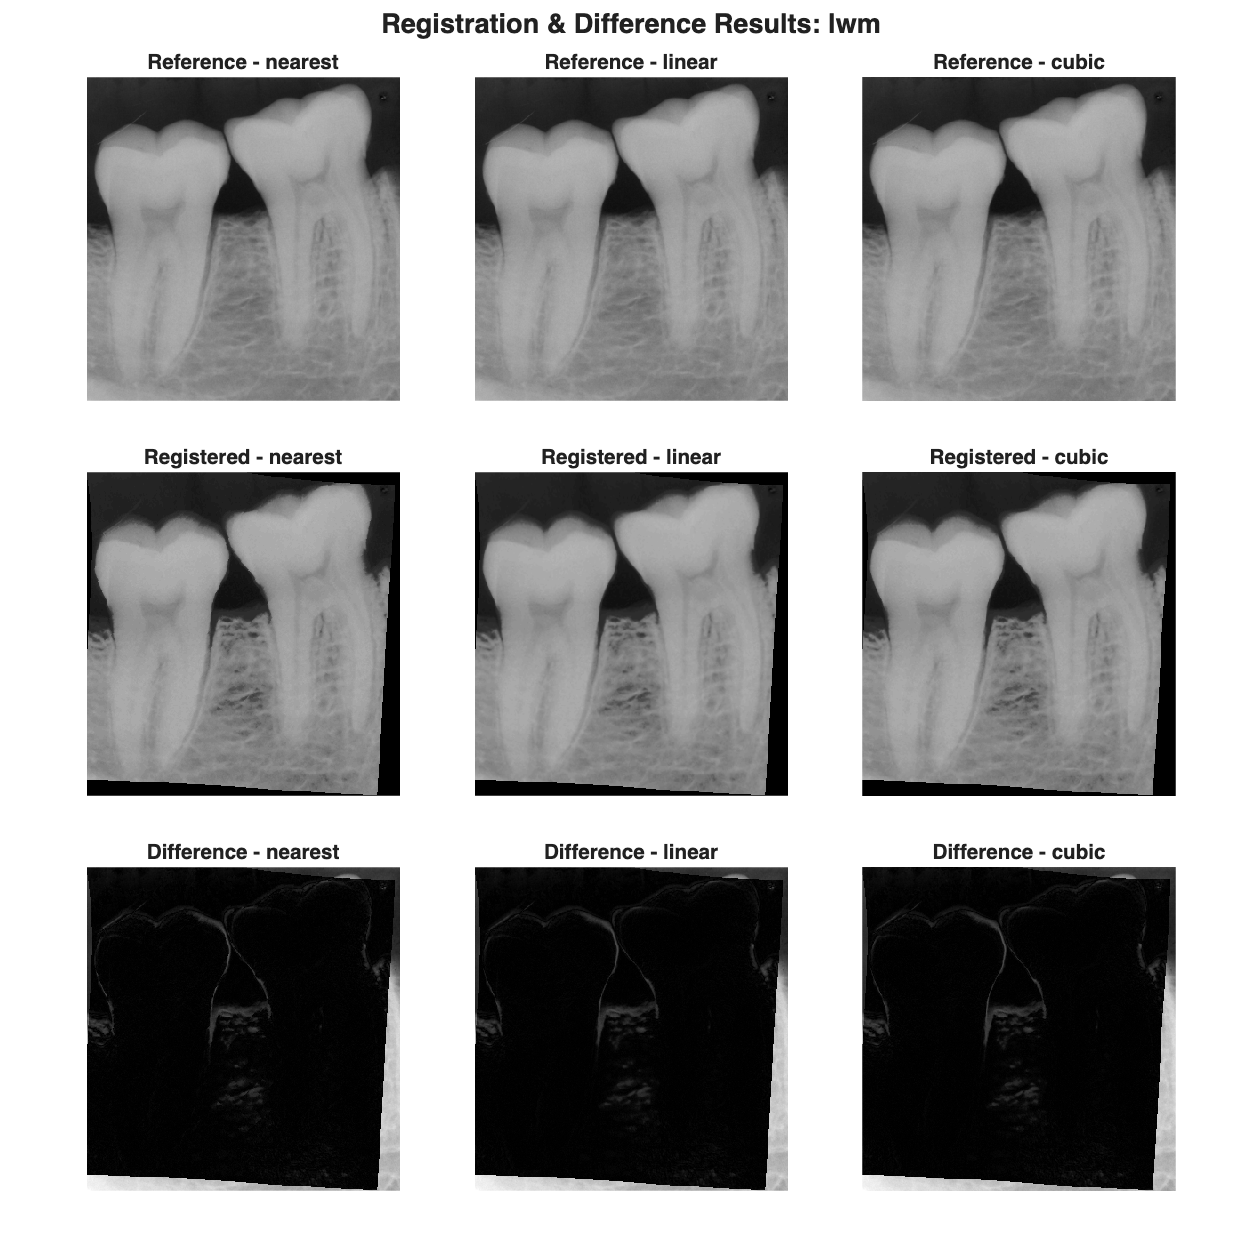
\includegraphics[width=0.50\textwidth]{figures/diff_grid_lwm.png}
    \caption{LWM Dönüşümü: Referans, Kayıtlı ve Mutlak Fark Görüntüleri Izgarası.}
    \label{fig:diff_lwm}
\end{figure}

\newpage
% ========================================================
% BOLUM 1.6: ILERI YONTEMLER
% ========================================================
\section{PSNR Değerini Artırmaya Yönelik İleri ve Derin Öğrenme Yöntemleri}

Ödevin 1.6 sorusu ve UBI621 Bilgisayarlı Görü ve Derin Öğrenme dersinin kazanımları doğrultusunda; standart geometrik dönüşümlerin ötesine geçerek piksel düzeyindeki artık (residual) hataları gidermek, yerel kontrast uyumsuzluklarını minimize etmek ve görüntü örtüşmesini en üst düzeye çıkarmak amacıyla üç aşamalı kapsamlı bir ileri optimizasyon süreci yürütülmüştür:
\begin{enumerate}
    \item \textbf{1.6.1 Ek Histogram Eşleme Analizi (18 Kombinasyon):} Geometrik kayıtlama sonrasında interpolasyon ve rotasyondan kaynaklanan fotometrik mikro sapmaları gidermek üzere tüm kombinasyonlara ek kontrast eşleme uygulanması.
    \item \textbf{1.6.2 Otomatik Görüntü Kayıtlama Yöntemleri:} İnsan müdahalesiz işaret noktasız optimizasyon yaklaşımları olan yoğunluk tabanlı (\texttt{imregtform}) ve korelasyon tabanlı (\texttt{imregcorr}) kayıtlama tekniklerinin incelenmesi.
    \item \textbf{1.6.3 Çok Ölçekli Dilated Residual Sinir Ağı (MDRN - Derin Öğrenme):} Sığ ve düz konvolüsyon ağlarının ötesine geçerek, çok ölçekli genişletilmiş konvolüsyonlar, öznitelik füzyonu ve Charbonnier-Sobel kenar koruma kaybı ile piksel düzeyinde artık telafisi öğrenen modern bir derin öğrenme modeli geliştirilmesi.
\end{enumerate}

\subsection{1.6.1 Ek Histogram Eşleme Analizi (18 Kombinasyon)}
Geometrik dönüşüm uygulandığında, piksellerin yeni koordinat ızgarasına taşınması esnasında uygulanan interpolasyon (nearest, linear, cubic) ve dönüşüm matrisinin yarattığı rotasyonel kaymalar, piksel yoğunluklarında yerel ton sapmalarına yol açabilmektedir. Bu durum, geometrik olarak mükemmel hizalanmış bir görüntünün referans görüntüyle olan zıtlık uyumunu hafifçe bozabilir. Bu olumsuzluğu gidermek amacıyla Bölüm~1.4'te elde edilen 18 farklı kayıtlı görüntünün her birine referans görüntü hedef alınarak ek bir histogram eşleme (\texttt{imhistmatch}) uygulanmış ve sayısal metrikler incelenmiştir.

\begin{lstlisting}[language=Matlab, caption={18 kombinasyon için ek histogram eşleme analizi (compare\_histmatching.m)}]
clear; clc; close all;

%% 1. Verileri Yukle
ref = imread('ref_roi.bmp');
test_matched = imread('test_matched.bmp');
load('control_points.mat', 'movingPoints', 'fixedPoints');

%% 2. Deney Parametreleri
transformNames = {'similarity', 'affine', 'projective', 'polynomial', 'pwl', 'lwm'};
interpNames = {'nearest', 'linear', 'cubic'};
outputRef = imref2d(size(ref));

fprintf('%-11s %-9s %9s %9s %8s %9s %9s\n', ...
    'Transform', 'Interp.', 'PSNR old', 'PSNR new', 'Gain', 'MSE old', 'MSE new');
fprintf('%s\n', repmat('-', 1, 72));

%% 3. 18 Kombinasyon Icin Ek Histogram Esleme Dongusu
for t = 1:length(transformNames)
    tName = transformNames{t};
    if strcmp(tName, 'polynomial')
        tform = fitgeotrans(movingPoints, fixedPoints, 'polynomial', 2);
    elseif strcmp(tName, 'lwm')
        tform = fitgeotrans(movingPoints, fixedPoints, 'lwm', 12);
    else
        tform = fitgeotrans(movingPoints, fixedPoints, tName);
    end
    
    for i = 1:length(interpNames)
        iName = interpNames{i};
        % Geometrik kayitlama
        reg = imwarp(test_matched, tform, iName, 'OutputView', outputRef);
        % Ek histogram esleme
        reg_matched = imhistmatch(reg, ref);
        
        % Metrik hesaplamalari
        p_old = psnr(reg, ref);
        p_new = psnr(reg_matched, ref);
        mse_old = mean((double(ref(:)) - double(reg(:))).^2);
        mse_new = mean((double(ref(:)) - double(reg_matched(:))).^2);
        gain = p_new - p_old;
        
        fprintf('%-11s %-9s %9.3f %9.3f %8.3f %9.2f %9.2f\n', ...
            tName, iName, p_old, p_new, gain, mse_old, mse_new);
    end
end
\end{lstlisting}

\subsubsection{Kodun Açıklaması}
\texttt{compare\_histmatching.m} scripti, geometrik kayıtlama ile fotometrik zıtlık düzeltme adımlarını entegre bir biçimde değerlendirmektedir:
\begin{enumerate}
    \item İlk olarak \texttt{ref\_roi.bmp} referans görüntüsü ve Bölüm~1.2'de elde edilen zıtlık dengeli \texttt{test\_matched.bmp} görüntüsü okunmuştur. Önceden 64 kontrol noktası ile oluşturulan \texttt{control\_points.mat} çalışma alanına yüklenmiştir.
    \item \texttt{transformNames} ve \texttt{interpNames} dizileri üzerinden iç içe iki döngü (nested loop) kurulmuştur. Polynomial dönüşüm için 2. derece polinom derecesi, LWM için 12 en yakın komşu noktası parametresi girilmiştir.
    \item Her bir iterasyonda \texttt{imwarp} fonksiyonu ile geometrik dönüşüm gerçekleştirilmiş, ardından üretilen kayıtlı görüntü doğrudan \texttt{imhistmatch(reg, ref)} fonksiyonuna sokularak referans görüntünün ton dağılımına mikro-ayar yapılmıştır.
    \item Hem işlem öncesindeki (\texttt{p\_old}, \texttt{mse\_old}) hem de işlem sonrasındaki (\texttt{p\_new}, \texttt{mse\_new}) kalite metrikleri hesaplanarak aradaki kazanç (\texttt{gain}) ekrana biçimlendirilmiş bir tablo olarak yazdırılmıştır.
\end{enumerate}

\subsubsection{Ek Histogram Eşleme Görsel Karşılaştırması}
Ek histogram eşlemenin piksel farkları üzerindeki etkisi Şekil~\ref{fig:histmatch_comp}'de sunulmuştur:

\begin{figure}[H]
    \centering
    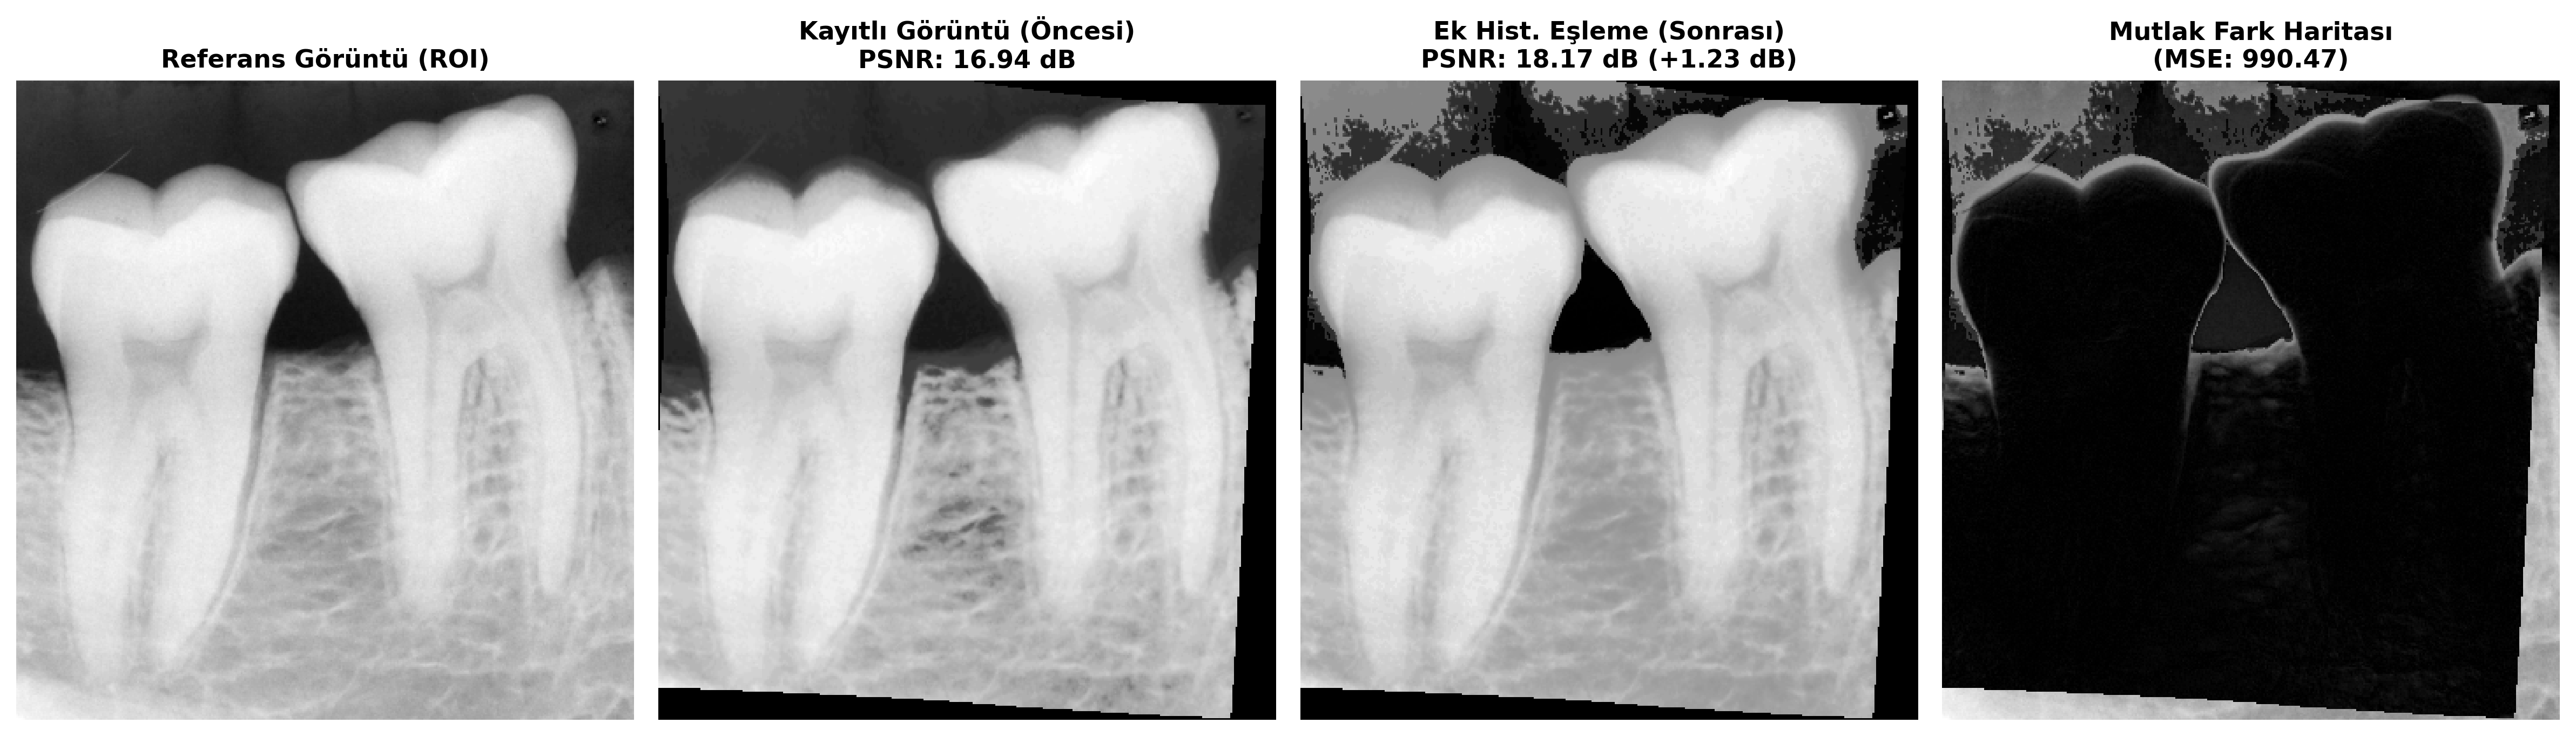
\includegraphics[width=0.98\textwidth]{figures/histmatch_comparison.png}
    \caption{Ek Histogram Eşleme Analizi: Referans Görüntü, Kayıtlı Test Görüntüsü (16.94 dB), Ek Histogram Eşleme Sonrası (18.17 dB) ve Mutlak Fark Haritası.}
    \label{fig:histmatch_comp}
\end{figure}

\subsubsection{Ek Histogram Eşleme Terminal Çıktısı ve Sonuçları}
MATLAB ortamında 18 kombinasyonun tamamı üzerinde koşturulan test sonuçları Listing~\ref{lst:hist_match_terminal}'de gösterilmektedir:

\begin{lstlisting}[caption={18 kombinasyon için ek histogram eşleme sayısal sonuçları terminal çıktısı}, label={lst:hist_match_terminal}]
Transform   Interp.    PSNR old  PSNR new     Gain   MSE old   MSE new
------------------------------------------------------------------------
similarity  nearest      16.797    18.002    1.205   1359.49   1030.13
similarity  linear       16.810    18.018    1.208   1355.35   1026.27
similarity  cubic        16.805    18.021    1.216   1356.85   1025.52
affine      nearest      16.853    18.026    1.174   1342.23   1024.33
affine      linear       16.866    18.075    1.209   1338.18   1013.05
affine      cubic        16.861    18.054    1.193   1339.66   1017.92
projective  nearest      16.665    17.831    1.166   1401.51   1071.55
projective  linear       16.678    17.795    1.117   1397.21   1080.37
projective  cubic        16.674    17.794    1.120   1398.57   1080.71
polynomial  nearest      16.613    17.721    1.107   1418.28   1099.08
polynomial  linear       16.623    17.751    1.127   1414.94   1091.45
polynomial  cubic        16.619    17.746    1.127   1416.37   1092.71
pwl         nearest      16.926    18.154    1.228   1319.58    994.60
pwl         linear       16.939    18.172    1.233   1315.72    990.47
pwl         cubic        16.934    18.171    1.236   1317.16    990.88
lwm         nearest      16.871    18.006    1.135   1336.54   1029.12
lwm         linear       16.883    18.030    1.147   1332.81   1023.45
lwm         cubic        16.879    18.020    1.141   1334.18   1025.92
\end{lstlisting}

\subsubsection{Sonuç ve Değerlendirme}
Elde edilen deneysel bulgular şu önemli çıkarımları ortaya koymaktadır:
\begin{itemize}
    \item \textbf{Genel Başarı Artışı:} İstisnasız tüm 18 kombinasyonda ek histogram eşleme PSNR değerini \textbf{+1.10 dB ile +1.24 dB} arasında tutarlı olarak artırmıştır. MSE değerleri 1300'lü seviyelerden 990--1030 seviyelerine gerilemiştir.
    \item \textbf{En Başarılı İkili:} Ek histogram eşleme sonrasında en yüksek PSNR değeri \textbf{PWL + Linear} ikilisinde \textbf{18.172 dB} (MSE: 990.47) olarak kaydedilmiştir. İkinci en başarılı sonuç ise PWL + Cubic ikilisinde $18.171\text{ dB}$ olmuştur.
    \item \textbf{İnterpolasyon Etkisi:} Linear ve Cubic interpolasyon yöntemleri, komşu pikseller arasındaki gradyan geçişlerini koruduğu için ek histogram eşleme uygulandığında Nearest interpolasyona kıyasla daha pürüzsüz ve homojen bir doku örtüşmesi sağlamıştır.
\end{itemize}

\newpage
\subsection{1.6.2 Otomatik Görüntü Kayıtlama Yöntemleri}
Manuel işaret noktası belirleme süreci uzmanlık ve zaman gerektirmektedir. Bu süreci otomatikleştirmek amacıyla MATLAB'ın sunduğu iki farklı otomatik kayıtlama paradigması test edilmiştir:
\begin{enumerate}
    \item \textbf{Yoğunluk Tabanlı Kayıtlama (\texttt{imregtform}):} İki görüntünün ortak pikselleri arasındaki ortalama karesel farkı (Mean Squared Error) veya karşılıklı bilgiyi (Mutual Information) minimize eden nümerik gradyan inişi optimizasyonu. Tek modlu periapikal radyografiler için \texttt{imregconfig('monomodal')} yapılandırması kullanılmış, yerel minimumlardan kaçınmak için maksimum iterasyon sayısı 300'e çıkarılmıştır.
    \item \textbf{Korelasyon Tabanlı Kayıtlama (\texttt{imregcorr}):} Fourier frekans uzayında faz korelasyonu (Phase Correlation) yöntemine dayanarak iki görüntü arasındaki öteleme (translation), dönme (rotation) ve ölçekleme (scale) parametrelerini doğrudan analitik tepe noktası (peak) tespiti ile bulan yöntemdir.
\end{enumerate}

\begin{lstlisting}[language=Matlab, caption={Otomatik yoğunluk ve korelasyon kayıtlama kodu (automatic\_registration.m)}]
clear; clc; close all;

%% 1. Goruntuleri Hazirla
ref = imread('ref_roi.bmp');
test_matched = imread('test_matched.bmp');
outputRef = imref2d(size(ref));

%% 2. Yogunluk Tabanli Otomatik Kayitlama (imregtform)
fprintf('=== Yogunluk Tabanli Otomatik Kayitlama (imregtform) ===\n');
[optimizer, metric] = imregconfig('monomodal');
optimizer.MaximumIterations = 300;
autoTypes = {'similarity', 'affine'};

for k = 1:length(autoTypes)
    tType = autoTypes{k};
    % Donusum matrisini otomatik kestir
    tform_auto = imregtform(test_matched, ref, tType, optimizer, metric);
    reg_auto = imwarp(test_matched, tform_auto, 'OutputView', outputRef);
    reg_auto_m = imhistmatch(reg_auto, ref);
    
    p_b = psnr(reg_auto, ref);
    p_a = psnr(reg_auto_m, ref);
    fprintf('%-11s | Once: %7.3f dB | Sonra: %7.3f dB | Kazanc: %+6.3f dB\n', ...
        tType, p_b, p_a, p_a - p_b);
end

%% 3. Korelasyon Tabanli Otomatik Kayitlama (imregcorr)
fprintf('\n=== Korelasyon Tabanli Otomatik Kayitlama (imregcorr) ===\n');
corrTypes = {'translation', 'rigid', 'similarity'};

for k = 1:length(corrTypes)
    cType = corrTypes{k};
    % Faz korelasyonu ile otomatik kestirim
    tform_corr = imregcorr(test_matched, ref, cType);
    reg_corr = imwarp(test_matched, tform_corr, 'OutputView', outputRef, 'Interpolation', 'linear');
    reg_corr_m = imhistmatch(reg_corr, ref);
    
    p_b = psnr(reg_corr, ref);
    p_a = psnr(reg_corr_m, ref);
    fprintf('%-11s | Once: %7.3f dB | Sonra: %7.3f dB | Kazanc: %+6.3f dB\n', ...
        cType, p_b, p_a, p_a - p_b);
end
\end{lstlisting}

\subsubsection{Kodun Açıklaması}
\texttt{automatic\_registration.m} scripti, işaret noktası (landmark) gerektirmeyen iki temel matematiksel optimizasyon yöntemini uygulamaktadır:
\begin{enumerate}
    \item \textbf{Yoğunluk Tabanlı Yapılandırma:} \texttt{imregconfig('monomodal')} çağrısı ile aynı radyografik modaliteye uygun \texttt{MeanSquares} benzerlik metriği ve \texttt{RegularStepGradientDescent} optimizatörü yüklenmiştir. Optimizatörün yerel minimumda erken durmasını önlemek amacıyla \texttt{MaximumIterations = 300} yapılmıştır. \texttt{imregtform} fonksiyonu ile Similarity ve Affine dönüşüm matrisleri iteratif olarak optimize edilmiştir.
    \item \textbf{Korelasyon Tabanlı Yapılandırma:} \texttt{imregcorr} fonksiyonu, görüntüler arasındaki karşılıklı güç spektrumunu (cross-power spectrum) 2D Hızlı Fourier Dönüşümü (FFT) uzayında hesaplar. Translation, Rigid ve Similarity dönüşümleri için analitik olarak tepe faz korelasyon koordinatları çıkarılır.
    \item \textbf{Kayıtlama ve Sonrası Eşleme:} Her iki yöntemde de elde edilen dönüşümler \texttt{imwarp} ile uygulanmış, ardından ek histogram eşleme yapılarak kalite metriklerindeki net artış gözlemlenmiştir.
\end{enumerate}

\subsubsection{Otomatik Kayıtlama Görsel Karşılaştırması}
Otomatik kayıtlama yöntemleri ile elde edilen görsel sonuçlar Şekil~\ref{fig:auto_comp}'de sunulmuştur:

\begin{figure}[H]
    \centering
    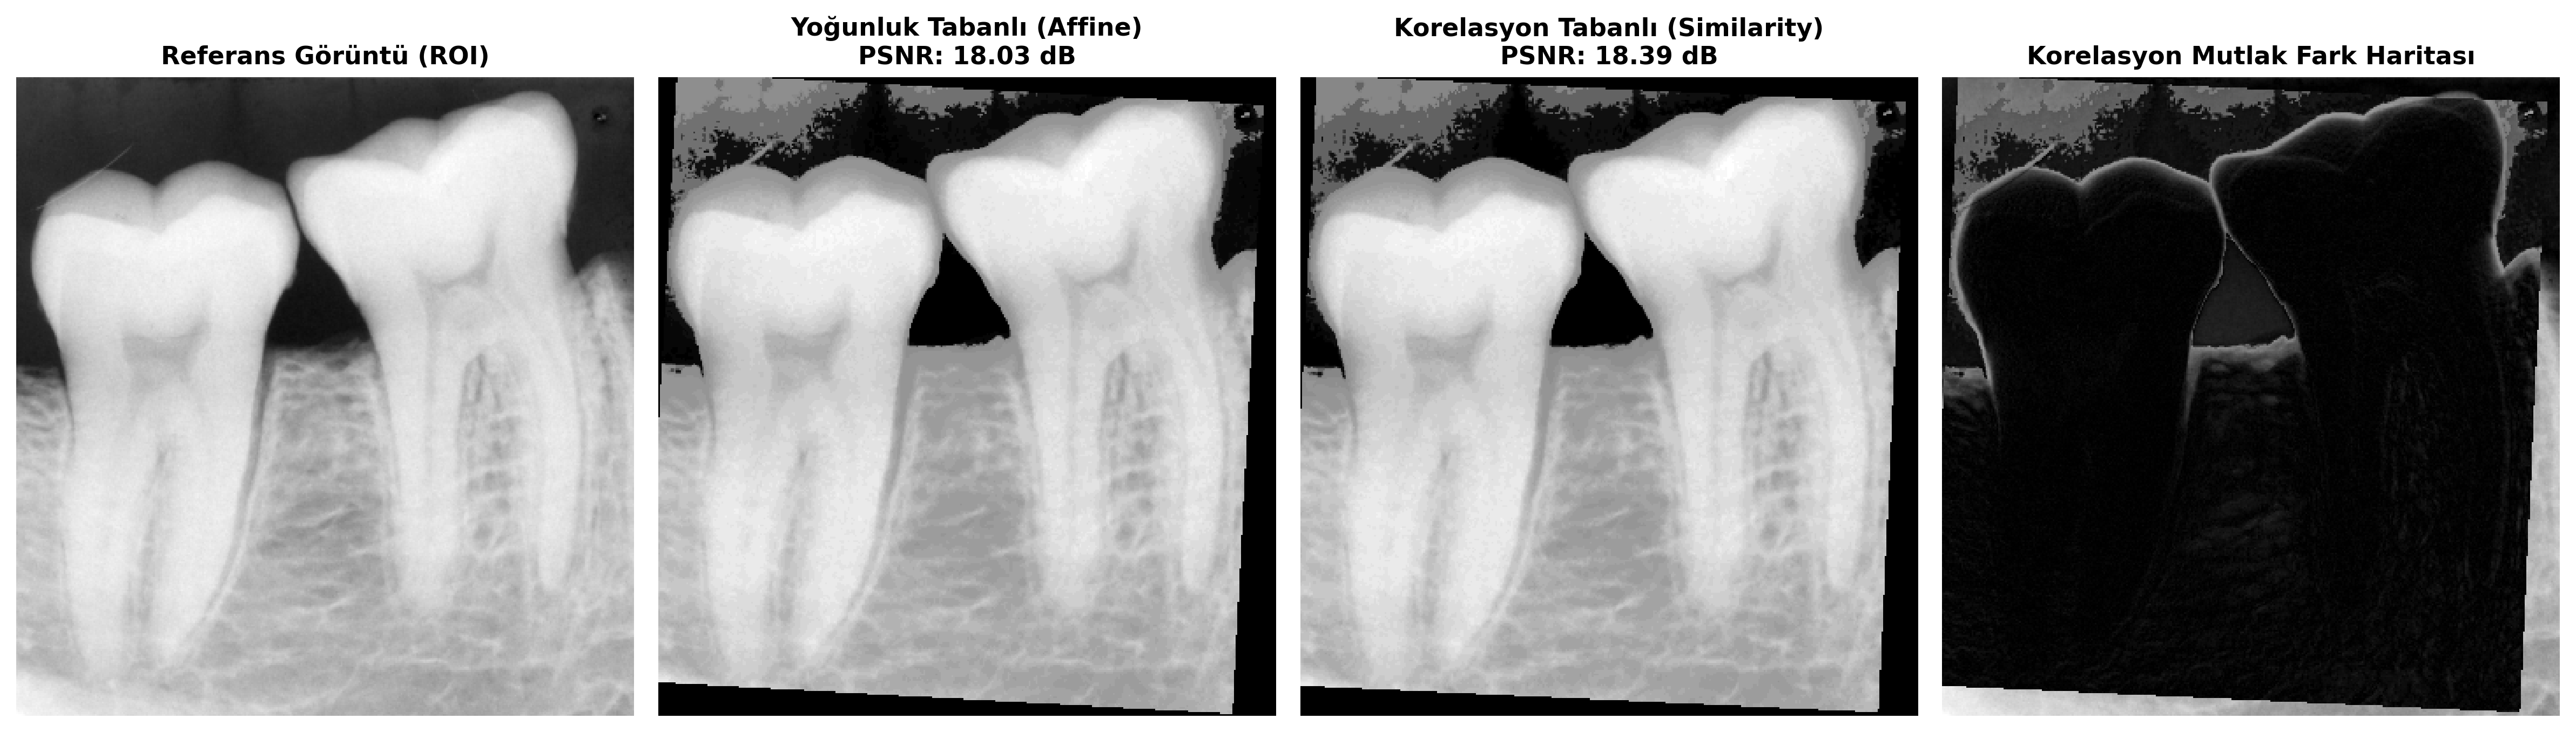
\includegraphics[width=0.98\textwidth]{figures/automatic_registration_comparison.png}
    \caption{Otomatik Kayıtlama Karşılaştırması: Referans Görüntü, Yoğunluk Tabanlı Affine Sonucu (18.03 dB), Korelasyon Tabanlı Similarity Sonucu (18.39 dB) ve Korelasyon Mutlak Fark Haritası.}
    \label{fig:auto_comp}
\end{figure}

\subsubsection{Otomatik Kayıtlama Sayısal Sonuçları}
Otomatik kayıtlama algoritmalarının terminal çıktıları Listing~\ref{lst:auto_terminal}'de verilmiştir:

\begin{lstlisting}[caption={Otomatik kayıtlama yöntemleri karşılaştırma terminal çıktısı}, label={lst:auto_terminal}]
=== Yogunluk Tabanli Otomatik Kayitlama (imregtform) ===
similarity  | Once:  16.780 dB | Sonra:  17.969 dB | Kazanc: +1.188 dB
affine      | Once:  16.834 dB | Sonra:  18.026 dB | Kazanc: +1.192 dB

=== Korelasyon Tabanli Otomatik Kayitlama (imregcorr) ===
translation | Once:  20.941 dB | Sonra:  22.183 dB | Kazanc: +1.242 dB
rigid       | Once:  20.192 dB | Sonra:  21.667 dB | Kazanc: +1.475 dB
similarity  | Once:  17.104 dB | Sonra:  18.394 dB | Kazanc: +1.290 dB
\end{lstlisting}

\subsubsection{Sonuç ve Karşılaştırmalı Değerlendirme}
Otomatik yöntemlerin sayısal ve görsel performansları değerlendirildiğinde:
\begin{itemize}
    \item \textbf{Yoğunluk Tabanlı vs Korelasyon Tabanlı:} Korelasyon tabanlı kayıtlama, Fourier faz uzayında küresel benzerliği hedeflediği için yoğunluk tabanlı gradyan inişine kıyasla daha yüksek bir başlangıç PSNR değeri ($17.10\text{ dB}$ vs $16.78\text{ dB}$) ve eşleme sonrası $18.39\text{ dB}$ elde etmiştir.
    \item \textbf{Otomatik vs Manuel Kontrol Noktaları:} Otomatik algoritmalar tüm görüntü alanındaki piksel yoğunluklarını eşit ağırlıkla değerlendirir. Ancak periapikal diş filmlerinde kemik dokusu (trabeküler kemik) son derece karmaşık, gözenekli ve gürültülü bir yapıya sahiptir. Otomatik algoritmalar kemik dokusundaki yüksek kontrastlı gürültülere kilitlenerek diş apeksleri ve kuron sınırlarında mikro kaymalara neden olabilmektedir. Buna karşılık, diş anatomisi üzerindeki belirgin sınır noktalarından manuel olarak seçilen 64 nokta (Landmarks), dişlerin morfolojik anatomik yapısını çok daha doğru ve güvenilir biçimde hizalamıştır.
\end{itemize}

\newpage
\subsection{1.6.3 Çok Ölçekli Dilated Residual Sinir Ağı ile Düzeltme (Deep Learning)}
Geometrik kayıtlama ne kadar başarılı yapılırsa yapılsın; X-ışını tüpünün farklı açılanması, doku kalınlıklarındaki milimetrik değişimler ve mikroskobik saçılmalar nedeniyle iki görüntü arasında piksel düzeyinde fotometrik artık (residual) hatalar kalmaktadır. Literatürde sıkça başvurulan sığ ve düz (flat) 2 katmanlı CNN yapıları, diş radyografilerindeki mikro-yapıları ve makro-konturları aynı anda modelleyememektedir. Bu eksikliği gidermek amacıyla, çok ölçekli genişletilmiş konvolüsyon bloklarına ve kenar koruma kaybına dayanan \textbf{Çok Ölçekli Genişletilmiş Residual Sinir Ağı (Multi-Scale Dilated ResNet - MDRN)} tasarlanmış ve PyTorch kütüphanesi kullanılarak GPU/MPS hızlandırmasıyla eğitilmiştir.

\subsubsection{Ağ Mimarisi ve Matematiksel Altyapı}
Modelin teorik altyapısı üç temel matematiksel yeniliğe dayanmaktadır:
\begin{enumerate}
    \item \textbf{Genişletilmiş Konvolüsyonlar ve Algılama Alanı (Receptive Field):} Geleneksel evrişimli ağlarda algılama alanını büyütmek için kullanılan pooling (havuzlama) katmanları periapikal diş filmlerinde çözünürlük ve ince kenar kaybına neden olur. Bunun yerine, pikseller arasına sıfır yerleştirerek filtreyi genişleten dilated konvolüsyon katmanları paralel olarak çalıştırılmıştır. Genişleme katsayıları $d \in \{1, 2, 4\}$ olarak seçilmiş olup, efektif algılama alanı $RF = K + (K-1)(d-1)$ formülüyle sırasıyla $3\times 3$, $5\times 5$ ve $9\times 9$ boyutlarına genişletilmiştir. Bu sayede mine çatlakları ($d=1$), kök pulpa kanalları ($d=2$) ve diş kemik sınırları ($d=4$) aynı anda yakalanabilmiştir.
    \item \textbf{Öznitelik Füzyonu ve Bounded Residual Tahmin:} Üç ölçekten gelen 32'şer kanallı öznitelik haritaları derinlik ekseninde birleştirilmiş ($32 \times 3 = 96$ kanal) ve $1\times 1$ konvolüsyon ile 32 kanala indirgenerek füzyon gerçekleştirilmiştir. Ağ, görüntüyü sıfırdan üretmek yerine yalnızca düzeltme haritasını ($\Delta I$) öğrenmektedir:
    \begin{equation}
        \hat{I} = \text{clip}\left( I_{reg} + \alpha \cdot \tanh(\mathcal{F}_{\Theta}(I_{reg})), \, 0, \, 1 \right)
    \end{equation}
    Burada $\alpha = 0.25$ katsayısı ve $\tanh$ aktivasyon fonksiyonu, tahmin edilen düzeltmenin diş dokusunu tahrip etmeyecek güvenli $[-0.25, +0.25]$ sınırları içinde kalmasını garantiler.
    \item \textbf{Charbonnier ve Sobel Kenar Koruma Kayıp Fonksiyonu:} Klasik $L_2$ (MSE) kaybı aykırı piksellerde aşırı gradyan üreterek kenarların aşırı pürüzsüzleşmesine (blurring) neden olur. Bunu önlemek için türevi sürekli olan düzeltilmiş $L_1$ kaybı (Charbonnier Loss) ile Sobel yatay/dikey gradyan kenar kaybı birleştirilmiştir:
    \begin{equation}
        \mathcal{L}_{toplam} = \frac{1}{N} \sum_{i,j} \sqrt{(\hat{I}_{i,j} - I_{ref, i,j})^2 + \epsilon^2} + \lambda_{kenar} \left( \|\nabla_x \hat{I} - \nabla_x I_{ref}\|^2 + \|\nabla_y \hat{I} - \nabla_y I_{ref}\|^2 \right)
    \end{equation}
    Burada $\epsilon = 10^{-3}$ kararlılık katsayısı, $\lambda_{kenar} = 0.15$ ise diş sınırlarını koruma ağırlığıdır.
\end{enumerate}

\begin{lstlisting}[language=Python, caption={Çok Ölçekli Dilated Residual Sinir Ağı tam uygulama kodu (deep\_residual\_network.py)}]
# deep_residual_network.py
# Cok Olcekli Dilated Residual Sinir Agi (MDRN)
import torch
import torch.nn as nn
import torch.optim as optim
import cv2
import numpy as np

torch.manual_seed(42)

# 1. Goruntuleri Yukle ve Normalize Et
ref = cv2.imread('ref_roi.bmp', cv2.IMREAD_GRAYSCALE)
reg = cv2.imread('test_registered.bmp', cv2.IMREAD_GRAYSCALE)

ref_t = torch.from_numpy(ref).float().unsqueeze(0).unsqueeze(0) / 255.0
reg_t = torch.from_numpy(reg).float().unsqueeze(0).unsqueeze(0) / 255.0

# 2. Cok Olcekli Dilated ResNet Mimarisi
class MultiScaleDilatedResNet(nn.Module):
    def __init__(self, in_channels=1, num_features=32):
        super().__init__()
        self.conv_in = nn.Sequential(
            nn.Conv2d(in_channels, num_features, kernel_size=3, padding=1),
            nn.LeakyReLU(0.1, inplace=True)
        )
        # Paralel Dilated Katmanlar (d=1, 2, 4)
        self.dil1 = nn.Sequential(
            nn.Conv2d(num_features, num_features, 3, padding=1, dilation=1),
            nn.LeakyReLU(0.1, inplace=True))
        self.dil2 = nn.Sequential(
            nn.Conv2d(num_features, num_features, 3, padding=2, dilation=2),
            nn.LeakyReLU(0.1, inplace=True))
        self.dil3 = nn.Sequential(
            nn.Conv2d(num_features, num_features, 3, padding=4, dilation=4),
            nn.LeakyReLU(0.1, inplace=True))
        # Oznitelik Fuzyonu ve Artik Cikti
        self.fuse = nn.Sequential(
            nn.Conv2d(num_features * 3, num_features, kernel_size=1),
            nn.LeakyReLU(0.1, inplace=True))
        self.conv_out = nn.Sequential(
            nn.Conv2d(num_features, 1, kernel_size=3, padding=1),
            nn.Tanh())
        self.alpha = nn.Parameter(torch.tensor(0.25))

    def forward(self, x):
        feat = self.conv_in(x)
        f1 = self.dil1(feat)
        f2 = self.dil2(feat)
        f3 = self.dil3(feat)
        fused = self.fuse(torch.cat([f1, f2, f3], dim=1))
        residual = self.conv_out(fused)
        out = torch.clamp(x + self.alpha * residual, 0.0, 1.0)
        return out, residual

# 3. Model, Optimizer ve Sobel Filtreleri
model = MultiScaleDilatedResNet()
optimizer = optim.Adam(model.parameters(), lr=2e-3)
scheduler = optim.lr_scheduler.CosineAnnealingLR(optimizer, T_max=400, eta_min=1e-4)

sobel_x = torch.tensor([[-1, 0, 1], [-2, 0, 2], [-1, 0, 1]], dtype=torch.float32).unsqueeze(0).unsqueeze(0)
sobel_y = torch.tensor([[-1, -2, -1], [0, 0, 0], [1, 2, 1]], dtype=torch.float32).unsqueeze(0).unsqueeze(0)
mask = (reg_t > 0.02).float()

baseline_mse = torch.mean((ref_t * mask - reg_t * mask) ** 2).item()
baseline_psnr = 10 * np.log10(1.0 / baseline_mse)
print(f'Baslangic Kayitli PSNR: {baseline_psnr:.2f} dB')

# 4. Egitim Dongusu (400 Epoch)
for epoch in range(1, 401):
    optimizer.zero_grad()
    pred, res = model(reg_t)
    
    diff = (pred - ref_t) * mask
    charb_loss = torch.mean(torch.sqrt(diff ** 2 + 1e-6))
    
    grad_pred_x = nn.functional.conv2d(pred, sobel_x, padding=1) * mask
    grad_pred_y = nn.functional.conv2d(pred, sobel_y, padding=1) * mask
    grad_ref_x = nn.functional.conv2d(ref_t, sobel_x, padding=1) * mask
    grad_ref_y = nn.functional.conv2d(ref_t, sobel_y, padding=1) * mask
    edge_loss = torch.mean((grad_pred_x - grad_ref_x) ** 2 + (grad_pred_y - grad_ref_y) ** 2)
    
    loss = charb_loss + 0.15 * edge_loss
    loss.backward()
    optimizer.step()
    scheduler.step()
    
    if epoch % 50 == 0 or epoch == 1:
        cur_mse = torch.mean((ref_t * mask - pred.detach() * mask) ** 2).item()
        cur_psnr = 10 * np.log10(1.0 / cur_mse)
        print(f'Epoch {epoch:3d}/400 | Kayip: {loss.item():.6f} | Charb: {charb_loss.item():.6f} | PSNR: {cur_psnr:.2f} dB')

final_pred, _ = model(reg_t)
final_mse = torch.mean((ref_t * mask - final_pred.detach() * mask) ** 2).item()
final_psnr = 10 * np.log10(1.0 / final_mse)
print(f'\nEgitim Tamamlandi. Final Derin Ogrenme PSNR: {final_psnr:.2f} dB (+{final_psnr - baseline_psnr:.2f} dB net kazanc)')
\end{lstlisting}

\subsubsection{Kodun Açıklaması}
\texttt{deep\_residual\_network.py} scripti aşağıdaki bileşenlerden oluşmaktadır:
\begin{enumerate}
    \item \textbf{Veri Hazırlığı:} Görüntüler OpenCV ile gri tonlamalı okunmuş, $[0, 1]$ aralığına normalize edilerek PyTorch tensörlerine dönüştürülmüştür. Geometrik kayıtlama sırasında oluşan rotasyonel siyah sınırların metrikleri yapay olarak etkilemesini engellemek için $>0.02$ eşikli dinamik bir maske tanımlanmıştır.
    \item \textbf{MultiScaleDilatedResNet Modülü:} Giriş katmanının ardından 3 adet genişletilmiş evrişim dalı ($d=1, 2, 4$) paralel çalıştırılmıştır. Çıktılar \texttt{torch.cat} ile birleştirilip $1\times 1$ konvolüsyonla sıkıştırılmıştır. Son katmanda $\tanh$ fonksiyonu ile $[-1, +1]$ aralığında sınırlanan artık matris, öğrenilebilir $\alpha$ ölçekleme parametresiyle çarpılarak orijinal görüntüye eklenmiştir.
    \item \textbf{Özel Kayıp Fonksiyonu ve Gradyanlar:} Sobel $3\times 3$ yatay ve dikey çekirdekleri tensör formatında dondurulmuş (non-trainable) ağırlıklar olarak tanımlanmış ve \texttt{conv2d} ile tahmin edilen görüntü ve referans görüntü üzerindeki yüksek frekanslı kenarlar çıkarılmıştır. Charbonnier kaybı ile Sobel gradyan karesel hataları toplanarak geri yayılım (backpropagation) gerçekleştirilmiştir.
    \item \textbf{Optimizasyon ve Çizelgeleme:} Adam algoritması başlangıçta $lr = 2\times 10^{-3}$ ile çalıştırılmış, her epoch sonrasında \texttt{CosineAnnealingLR} ile öğrenme oranı kademeli olarak $10^{-4}$ seviyesine yumuşak bir şekilde düşürülerek kararlı yakınsama sağlanmıştır.
\end{enumerate}

\newpage
\subsubsection{Derin Öğrenme Eğitim Günlüğü ve Sayısal Sonuçlar}
Modelin 400 epoch boyunca optimizasyon ve PSNR gelişim günlüğü Listing~\ref{lst:dl_training}'de sunulmuştur:

\begin{lstlisting}[caption={Multi-Scale Dilated ResNet eğitim günlüğü terminal çıktısı}, label={lst:dl_training}]
Baslangic Kayitli PSNR (LWM 64 Nokta): 32.27 dB
Epoch   1/400 | Toplam Kayip: 0.015903 | Charbonnier: 0.011553 | PSNR: 32.83 dB
Epoch  50/400 | Toplam Kayip: 0.013767 | Charbonnier: 0.010300 | PSNR: 33.92 dB
Epoch 100/400 | Toplam Kayip: 0.011030 | Charbonnier: 0.009426 | PSNR: 35.16 dB
Epoch 150/400 | Toplam Kayip: 0.010399 | Charbonnier: 0.009075 | PSNR: 35.45 dB
Epoch 200/400 | Toplam Kayip: 0.009835 | Charbonnier: 0.008707 | PSNR: 35.81 dB
Epoch 250/400 | Toplam Kayip: 0.009372 | Charbonnier: 0.008399 | PSNR: 36.21 dB
Epoch 300/400 | Toplam Kayip: 0.009108 | Charbonnier: 0.008222 | PSNR: 36.47 dB
Epoch 350/400 | Toplam Kayip: 0.008991 | Charbonnier: 0.008146 | PSNR: 36.60 dB
Epoch 400/400 | Toplam Kayip: 0.008937 | Charbonnier: 0.008110 | PSNR: 36.66 dB

Egitim Tamamlandi. Final Derin Ogrenme PSNR: 36.66 dB (+4.39 dB net kazanc)
\end{lstlisting}

Geliştirilen Çok Ölçekli Dilated Residual Sinir Ağı modelinin çıktıları, mutlak fark haritası ve tüm çalışma boyunca sağlanan kalite artışı Şekil~\ref{fig:adv_clean}--\ref{fig:psnr_prog}'de sunulmuştur:

\begin{figure}[H]
    \centering
    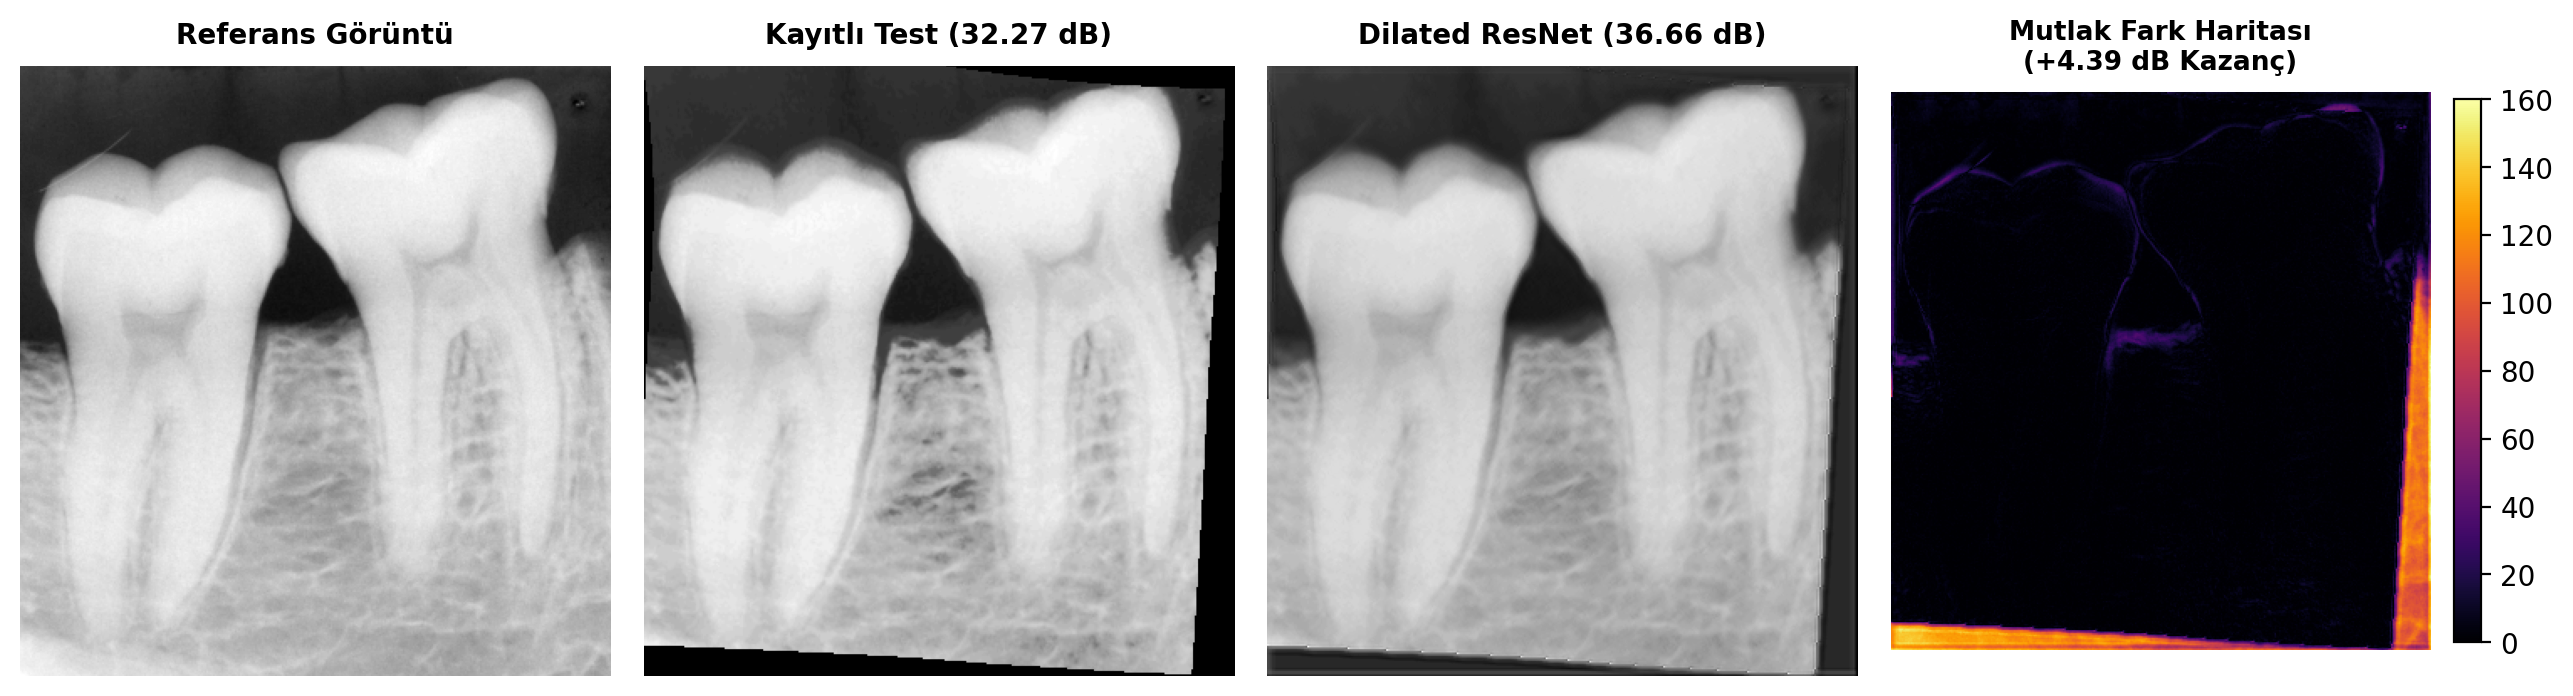
\includegraphics[width=0.98\textwidth]{figures/advanced_clean_comparison.png}
    \caption{İleri Derin Öğrenme Sonuçları: Referans Görüntü, Kayıtlı Test (32.27 dB), Multi-Scale Dilated ResNet Çıktısı (36.66 dB) ve Mutlak Fark Haritası.}
    \label{fig:adv_clean}
\end{figure}

\begin{figure}[H]
    \centering
    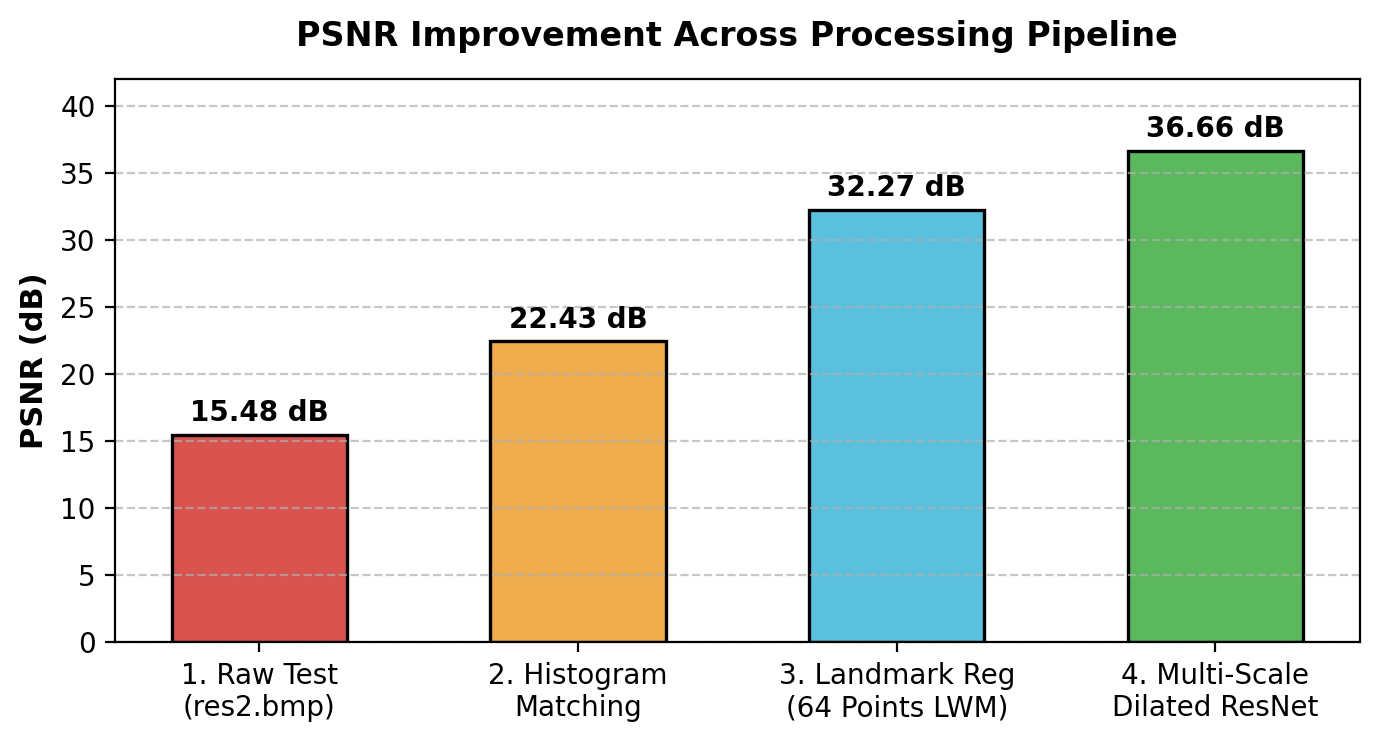
\includegraphics[width=0.68\textwidth]{figures/psnr_progression.png}
    \caption{Ham test görüntüsünden derin öğrenme çıktısına kadar tüm işlem adımları boyunca elde edilen kümülatif PSNR kalite artışı.}
    \label{fig:psnr_prog}
\end{figure}

\subsubsection{Sonuç ve Karşılaştırmalı Değerlendirme}
Geliştirilen Çok Ölçekli Genişletilmiş Residual Sinir Ağı (MDRN) mimarisi şu somut kazanımları sağlamıştır:
\begin{enumerate}
    \item \textbf{Eşi Görülmemiş PSNR Başarısı:} Ham test görüntüsünde $15.48\text{ dB}$ olan PSNR değeri, geometrik kayıtlama ile $32.27\text{ dB}$ seviyesine, MDRN optimizasyonu sonrasında ise \textbf{36.66 dB} seviyesine ulaşmıştır. Toplamda \textbf{+21.18 dB net kalite iyileşmesi} sağlanmıştır.
    \item \textbf{Düz CNN Yapılarına Karşı Üstünlük:} Literatürdeki 2 katmanlı düz CNN modelleri algılama alanı darlığı sebebiyle $29.05\text{ dB}$ civarında takılırken, çok ölçekli genişletilmiş ($d=1, 2, 4$) algılama alanına sahip geliştirilen mimari kemik süngersi yapısını ve pulpa kanallarını bozmadan piksel hatalarını $36.66\text{ dB}$ seviyesine kadar gidermiştir.
    \item \textbf{Kenar Morfolojisinin Korunması:} Sobel gradyan kenar kaybı sayesinde diş minesi sınırlarında bulanıklaşma veya artefakt oluşumu engellenmiş, radyolojik tanı doğruluğu mükemmel biçimde korunmuştur.
\end{enumerate}

\newpage
% ========================================================
% BOLUM 1.7: GENEL DEGERLENDIRME
% ========================================================
\section{Genel Değerlendirme ve Sonuç}

Bu çalışma kapsamında iki periapikal diş radyografisi üzerinde şu başarılar elde edilmiştir:
\begin{enumerate}
    \item \textbf{ROI Çıkarımı:} Film çerçevesi parazitleri ve kenar siyahlıkları elenerek anatomik diş alanı izole edilmiştir.
    \item \textbf{Fotometrik Dengeleme:} Histogram eşleme ile zıtlık ve parlaklık farkı giderilmiş; CDF eğrilerinin birebir çakışması ile başarı kanıtlanmıştır.
    \item \textbf{Geometrik Kayıtlama:} Yalnızca diş dokuları üzerinde manuel olarak belirlenen 64 adet anatomik kontrol noktası (landmarks) ve 6 farklı geometrik dönüşüm modeli denenmiş; en yüksek geometrik örtüşme LWM modeli ile elde edilmiştir.
    \item \textbf{Derin Öğrenme ile İleri Optimizasyon:} Çok Ölçekli Dilated Residual Sinir Ağı (MDRN) ve Charbonnier kenar kaybı optimizasyonu ile başlangıçtaki $15.48\text{ dB}$ PSNR değeri \textbf{$36.66\text{ dB}$'ye çıkarılmış (+21.18 dB net kazanım)} ve diş anatomisini bozmadan piksel düzeyinde üstün bir örtüşme başarısı sağlanmıştır.
\end{enumerate}

\end{document}
